% ch07_noisy_gates.tex by tools/conversion/make_ch07.py and since edited by hand (do not rerun it); see
% chapters/ch01_ch08_NOTES.md. The subsections of the former Section "Proofs and further results" are sections here.
\chapter{Noisy gates: proofs and further results}\label{gate:proofschapter}\label{gate:sec:proofs}
\chaptermark{Noisy gates: proofs}
\begingroup
\chapmacro[1]{\dn}{\|#1\|_\diamond}
\chapmacro{\Fg}{\hat F}
\chapmacro{\FU}{F_{\mathrm U}}
\chapmacro{\DBS}{D_{\mathrm{BS}}}
\chapmacro{\lmin}{\lambda_{\min}}
\chapmacro{\lmax}{\lambda_{\max}}
\chapmacro{\Id}{\mathbf 1}
\chapmacro{\Dp}{\mathcal D_p}
\chapmacro{\cN}{\mathcal N}
\chapmacro{\cA}{\mathcal A}
\chapmacro{\IR}{F_{\mathrm{RLD}}}
\chapmacro{\IB}{F_{\mathrm{BKM}}}
\chapmacro{\IS}{F_{\mathrm{SLD}}}
\chapmacro{\Iinf}{F_{\infty}}
\chapmacro{\ltil}{\tilde\lambda}
\chapmathop{\vect}{vec}

\begin{chaptersummary}
This chapter contains the proofs of the results stated in Chapter~\ref{gate:chapter} and the further results behind them: closed forms for Pauli channels, including biased noise and correlated miscalibrations, the amplitude-damping analysis, the local and finite-miscalibration comparisons of the converses with the adaptive Stein and Chernoff exponents, the certification bounds, the numerical methods, and the refinements of results of Chapters~\ref{cont:chapter}, \ref{shA:chapter} and~\ref{chn:chapter} that these proofs need.
\end{chaptersummary}

This chapter is the companion of Chapter~\ref{gate:chapter}, which states the results and their physical meaning; here we prove them. It contains the proofs of the statements made in Sections~\ref{gate:sec:setting}--\ref{gate:sec:cert} of Chapter~\ref{gate:chapter}, closed-form expressions for Pauli channels, the amplitude-damping analysis, the certification bounds and the numerical methods. It keeps the notation of Chapter~\ref{gate:chapter}, which Section~\ref{gate:sec:notation} recalls, and the theorems, equations, figures and tables of that chapter are cited by their numbers there, which begin with~\ref{gate:chapter}. Results proved in Chapters~\ref{cont:chapter}, \ref{shA:chapter} and~\ref{chn:chapter} are used by reference; Section~\ref{gate:smp:sec} collects the refinements of those results that are needed here, together with pointers to the rest. Statements labelled as conjectures are not claimed to be proved.

\section{Notation and conventions}\label{gate:sec:notation}

Channels $\Phi,\Psi$ map operators on $\mathcal X$ ($\dim\mathcal X=d_X$) to operators on $\mathcal Y$ ($\dim\mathcal Y=d_Y$). The unnormalized Choi matrix is $J(\Phi)=\sum_{ij}\Phi(|i\rangle\langle j|)\otimes|i\rangle\langle j|$, with output first, so that $\Tr J(\Phi)=d_X$ and $\Tr_{\mathcal Y}J(\Phi)=\Id$ for a channel. The Choi floor is $\lambda(\Phi)=\lmin(J(\Phi))$, and $\ltil=\lambda/d_X$ is the floor of the Choi state $J/d_X$. The diamond norm $\dn{\cdot}$ is unnormalized ($\dn{\Phi-\Psi}\le2$ for channels). We write $\vect(A)=\sum_{ij}A_{ij}|i\rangle|j\rangle$, so that $J(\mathrm{Ad}_A)=\vect(A)\vect(A)^\dagger$ with $\mathrm{Ad}_A(\rho)=A\rho A^\dagger$.

For positive definite $A,B$ and $s\in[0,1]$, $A\#_sB=A^{1/2}(A^{-1/2}BA^{-1/2})^sA^{1/2}$ is the weighted Kubo--Ando geometric mean~\cite{KuboAndo1980}, extended to positive semidefinite arguments by continuity from above, and $\#=\#_{1/2}$. The channel quantities are
\begin{gather}
\Fg(\Phi,\Psi)=\lmin\Tr_{\mathcal Y}[J(\Phi)\#J(\Psi)],\qquad \hat Q_s(\Phi\|\Psi)=\lmin\Tr_{\mathcal Y}[J(\Psi)\#_sJ(\Phi)],\notag\\
\hat C(\Phi,\Psi)=-\ln\inf_{s\in(0,1)}\hat Q_s,\\
\DBS(\Phi\|\Psi)=\lmax\Tr_{\mathcal Y}\big[J_\Phi^{1/2}\ln\big(J_\Phi^{1/2}J_\Psi^{-1}J_\Phi^{1/2}\big)J_\Phi^{1/2}\big],
\end{gather}
with $J_\Phi=J(\Phi)$~\cite{FangFawzi2021,KatariyaWilde2021} (Chapters~\ref{cont:chapter} and~\ref{chn:chapter}). The Umegaki channel divergence $D(\Phi\|\Psi)$ is the supremum over input states $\psi_{R X}$ of $D\big((\mathrm{id}\otimes\Phi)\psi\|(\mathrm{id}\otimes\Psi)\psi\big)$, and the Uhlmann channel root fidelity $\FU(\Phi,\Psi)$ is the minimum over inputs of $\|\sqrt{\omega}\sqrt{\sigma}\|_1$ for the two output states. The Thompson metric is $d_T(\Psi,\Psi')=\inf\{t:e^{-t}J(\Psi)\le J(\Psi')\le e^tJ(\Psi)\}$~\cite{Thompson1963}. Fisher informations are denoted $F_{\mathrm{RLD}}$, $F_{\mathrm{BKM}}$, $F_{\mathrm{SLD}}$ and $\Iinf$ for the asymptotic adaptive rate; the Uhlmann root fidelity is $\FU$.

For $n$ qubits, $\Dp(\rho)=(1-p)\rho+p\Tr(\rho)\Id/2$ acts on each qubit, and a Pauli channel is $\mathcal P_q(\rho)=\sum_Qq_QQ\rho Q$ with $Q$ ranging over the $d^2$ Pauli strings ($d=2^n$). Local depolarizing noise is $\Dp^{\otimes n}=\mathcal P_q$ with $q_Q=(1-\frac{3p}{4})^{n-\mathrm{wt}Q}(\frac p4)^{\mathrm{wt}Q}$, and global depolarizing noise is $\Dp^{\rm glob}(\rho)=(1-p)\rho+p\Tr(\rho)\Id/d$. The gate model is
\begin{equation}\label{gate:eq:Sgate}
\cN_\delta=\mathcal P_q\circ\mathrm{Ad}_{R_P(\delta)}\circ\mathrm{Ad}_U,\qquad R_P(\delta)=e^{-i\delta P/2},
\end{equation}
with $P\ne\Id$ a Pauli string of weight $w$, and $\cN_{p,\delta}$ denotes the case $\mathcal P_q=\Dp^{\otimes n}$. For the qubit examples we take $P=Z$; the choice $P=X$ gives identical values, because the two pairs differ by a common input and output unitary. For fixed $P$ the Pauli strings split into $d^2/2$ unordered pairs $\{Q,QP\}$, and for each pair we put
\begin{equation}\label{gate:eq:Sx}
x_Q(\delta)=\frac{(q_Q-q_{QP})^2\sin^2(\delta/2)}{4q_Qq_{QP}},\qquad g(x)=1-(1+x)^{-1/2},\qquad \varphi(x)=\sqrt{\frac{x}{1+x}}\,\operatorname{arsinh}\sqrt x .
\end{equation}

\section{Choi matrices and the diamond norm}\label{gate:sec:lemJ}

\begin{lemma}[cf.\ Lemma~\ref{cont:lem:choi vs cb}]\label{gate:lem:J}
Let $\mathcal M$ be a Hermitian-preserving map. Then $\|J(\mathcal M)\|_\infty\le\frac{d_X}{2}\dn{\mathcal M}+\frac12|\Tr J(\mathcal M)|\le d_X\dn{\mathcal M}$. In particular $\|J(\Phi)-J(\Phi')\|_\infty\le\frac{d_X}{2}\dn{\Phi-\Phi'}$ for channels. Both constants are attained in every dimension: by $\mathcal M=\mathrm{id}$ for $d_X$, and by $\mathrm{id}-\mathrm{Ad}_V$ with $\Tr V=0$, or by $\mathrm{id}-\mathcal D^{\rm glob}_1$, for $d_X/2$.
\end{lemma}

\begin{proof}
The inequalities and the cases $\mathcal M=\mathrm{id}$ and $\mathrm{id}-\mathrm{Ad}_V$ are Lemma~\ref{cont:lem:choi vs cb} in Chapter~\ref{cont:chapter}.
For $\mathrm{id}-\mathcal D_1^{\rm glob}$, $J=|\Omega\rangle\langle\Omega|-\Id/d$ has norm $d-1/d$, and writing $\mathcal D_1^{\rm glob}$ as the uniform mixture of the $d^2$ Weyl unitaries gives $\dn{\mathrm{id}-\mathcal D_1^{\rm glob}}\le2(1-d^{-2})$, so equality holds.
\end{proof}

Hence, if $\dn{\Psi'-\Psi}\le\epsilon$ and $J(\Psi)\ge\lambda\Id$, then $\|J(\Psi')-J(\Psi)\|_\infty\le r\lambda$ with $r=d_X\epsilon/(2\lambda)$, and
\begin{equation}\label{gate:eq:Ssandwich}
(1-r)J(\Psi)\le J(\Psi')\le(1+r)J(\Psi),\qquad d_T(\Psi,\Psi')\le\ln\frac1{1-r}\quad(r<1).
\end{equation}
The same holds with a Choi-state trace-norm hypothesis $\|J(\Psi)/d_X-J(\Psi')/d_X\|_1\le\epsilon$, since $\|X\|_\infty\le\frac12\|X\|_1$ for traceless Hermitian $X$.

\section{\texorpdfstring{The Choi-floor law (Theorem~\ref{gate:thm:floor})}{The Choi-floor law}}\label{gate:sec:floor}

\begin{proof}[Proof of Eq.~\eqref{gate:eq:floor}]
By Eq.~\eqref{gate:eq:Ssandwich} and joint monotonicity of $\#_s$ in each argument, $J(\Psi')\#_sJ(\Phi)$ lies between $[(1\mp r)J(\Psi)]\#_sJ(\Phi)=(1\mp r)^{1-s}\,J(\Psi)\#_sJ(\Phi)$. The map $Z\mapsto\lmin\Tr_{\mathcal Y}Z$ is monotone and positively homogeneous, so $(1-r)^{1-s}\hat Q_s(\Phi\|\Psi)\le\hat Q_s(\Phi\|\Psi')\le(1+r)^{1-s}\hat Q_s(\Phi\|\Psi)$. For $s=\frac12$ this is the statement for $\Fg$, and taking the minimum over $s$ gives $|\hat C(\Phi,\Psi')-\hat C(\Phi,\Psi)|\le\ln\frac1{1-r}$. No property of $J(\Phi)$ is used.
\end{proof}

\begin{proof}[Proof of the bound for $\DBS$ in Theorem~\ref{gate:thm:floor}]
Let $\Phi$ be a channel and let $P$ be the projection onto the support of $J_\Phi$. Put $X_\Psi=P J_\Phi^{1/2}J_\Psi^{-1}J_\Phi^{1/2}P$, regarded as a positive definite operator on $\mathrm{ran}\,P$. From $(1-r)J_\Psi\le J_{\Psi'}\le(1+r)J_\Psi$ and the operator monotonicity of inversion, $(1+r)^{-1}J_\Psi^{-1}\le J_{\Psi'}^{-1}\le(1-r)^{-1}J_\Psi^{-1}$, hence $(1+r)^{-1}X_\Psi\le X_{\Psi'}\le(1-r)^{-1}X_\Psi$. The logarithm is operator monotone, so $\ln X_\Psi-\ln(1+r)P\le\ln X_{\Psi'}\le\ln X_\Psi+\ln\frac1{1-r}P$. Conjugating with $J_\Phi^{1/2}$ preserves the order, and $J_\Phi^{1/2}PJ_\Phi^{1/2}=J_\Phi$. Taking $\Tr_{\mathcal Y}$, which is positive, and using $\Tr_{\mathcal Y}J_\Phi=\Id$ for a channel gives
\begin{equation*}
T_\Psi-\ln(1+r)\Id\le T_{\Psi'}\le T_\Psi+\ln\tfrac1{1-r}\Id,\qquad T_\Psi=\Tr_{\mathcal Y}\big[J_\Phi^{1/2}\ln(X_\Psi)J_\Phi^{1/2}\big],
\end{equation*}
and the largest eigenvalues of $T_\Psi$ and $T_{\Psi'}$ are the BS divergences. Since $\lmax$ is monotone and $\lmax(T+c\Id)=\lmax(T)+c$, $-\ln(1+r)\le\DBS(\Phi\|\Psi')-\DBS(\Phi\|\Psi)\le\ln\frac1{1-r}$. For a completely positive $\Phi$ the same argument gives the bound multiplied by $\|\Phi^*(\Id)\|_\infty$.
\end{proof}

\begin{proof}[Proof of the sharpness statement, Eq.~\eqref{gate:eq:sharp}]
The upper bound $d_X/(4\lambda)$ follows from Eq.~\eqref{gate:eq:floor} as $\epsilon\to0$. For the lower bound let $v_W=\vect(W)$, $W$ unitary, be a $\lambda$-eigenvector of $J(\Psi)$, so $\|v_W\|^2=d$, and let $\Phi=\mathrm{Ad}_W$. For $B>0$ the rank-one formula $v_Wv_W^\dagger\#B=v_Wv_W^\dagger/\langle v_W,B^{-1}v_W\rangle^{1/2}$ and $\Tr_{\mathcal Y}v_Wv_W^\dagger=\Id$ give $\Fg(\mathrm{Ad}_W,\Psi')=\langle v_W,J(\Psi')^{-1}v_W\rangle^{-1/2}$. Take any unitary $W'$ with $\Tr W^\dagger W'=0$ (it need not lie in the floor eigenspace), $\mathcal M=\frac12(\mathrm{Ad}_W-\mathrm{Ad}_{W'})$, which has $\dn{\mathcal M}=1$, and $\Psi_e=\Psi+e\mathcal M$, a channel for small $|e|$ because $J(\Psi)>0$. Then $J(\mathcal M)=\frac12(v_Wv_W^\dagger-v_{W'}v_{W'}^\dagger)$, $\frac{d}{de}\langle v_W,J(\Psi_e)^{-1}v_W\rangle|_{e=0}=-\lambda^{-2}\langle v_W,J(\mathcal M)v_W\rangle=-d^2/(2\lambda^2)$ and $\langle v_W,J(\Psi)^{-1}v_W\rangle=d/\lambda$. Hence $\frac{d}{de}\ln\Fg=\frac12\cdot\frac{d^2/(2\lambda^2)}{d/\lambda}=\frac{d}{4\lambda}$. For a Pauli channel $\mathcal P_q\circ\mathrm{Ad}_U$ the vectors $\vect(QU)$ are eigenvectors with eigenvalues $dq_Q$, so the floor eigenspace always contains such a $v_W$; for local noise $Q$ has full weight, which is the correlated error mentioned after Theorem~\ref{gate:thm:floor}.
\end{proof}

A numerical check in 40-digit arithmetic gives the ratio of the slope to $d/(4\lambda)$ as $1.0000000$ ($n=1$, $p=10^{-2}$), $1.0000034$ ($n=1$, $10^{-3}$), $0.9999816$ ($n=2$, $10^{-2}$) and $0.99999995$ ($n=2$, $10^{-3}$); a 60-digit finite difference confirms $d^2/(4p^n)$ for $n=1,2,3$ to $4\times10^{-10}$.

\emph{Two-sided version.} If both channels move, with $\eta_J=\max\{\|J(\Phi')-J(\Phi)\|_\infty,\|J(\Psi')-J(\Psi)\|_\infty\}$ and $\lambda=\min\{\lambda(\Phi),\lambda(\Psi)\}$, then $(1-\eta_J/\lambda)\Fg(\Phi,\Psi)\le\Fg(\Phi',\Psi')\le(1+\eta_J/\lambda)\Fg(\Phi,\Psi)$, and similarly for every Kubo--Ando connection (Theorem~\ref{cont:thm:choi floor} in Chapter~\ref{cont:chapter}; Proposition~\ref{gate:smp:prop:twosided} also allows separate floors). Since $\Fg$ is symmetric, Eq.~\eqref{gate:eq:sharp} shows that each of the two terms is sharp separately; whether the constant $d_X/(2\lambda)$ is attained when both channels move is open.

\begin{proposition}[Absolute slope at a qubit gate]\label{gate:prop:L2}
Let $\Psi=\Dp\circ\mathrm{Ad}_U$ on one qubit and $\Sigma(p)=\sup_\Phi\sup_{\mathcal M}|\frac{d}{de}\Fg(\Phi,\Psi+e\mathcal M)|_{e=0}$, over completely positive $\Phi$ and trace-annihilating $\mathcal M$ with $\dn{\mathcal M}=1$. Then $\frac{2}{3\sqrt3}\frac1p(1+o(1))\le\Sigma(p)\le\frac1p$. The lower bound is attained by unitary $\Phi$; the supremum over unitary $\Phi$ is
\begin{equation}
\Sigma_{\rm unit}(p)=\max_\theta\frac{\sqrt2}{4}\,\frac{\cos^2\theta/\beta^2+\sin^2\theta/\lambda^2}{(\cos^2\theta/\beta+\sin^2\theta/\lambda)^{3/2}},\qquad\beta=2-\tfrac{3p}{2},\ \lambda=\tfrac p2,
\end{equation}
with $p\,\Sigma_{\rm unit}=0.384904$ at $p=10^{-2}$ and $0.384900$ at $p=10^{-3},10^{-4}$.
\end{proposition}

\begin{proof}
The upper bound is Eq.~\eqref{gate:eq:floor} with $\Fg\le1$. For unitary $\Phi$ with Choi vector $v=\sqrt d(\cos\theta\,\hat e_{\Id}-i\sin\theta\,\hat e_P)$ in the eigenbasis of $J(\Psi)$, $\frac{d\Fg}{de}=\frac12\Fg^3\langle u,J(\mathcal M)u\rangle$ with $u=J(\Psi)^{-1}v$, which is proportional to the Choi vector of a unitary. Lemma~\ref{gate:lem:J} bounds $\langle u,J(\mathcal M)u\rangle\le\frac d2\|u\|^2$, with equality for $\mathcal M=\frac12(\mathrm{Ad}_{\hat u}-\mathrm{Ad}_{\hat u'})$. This gives $\Sigma_{\rm unit}$; with $\sin^2\theta=y\lambda/d$ and $p\to0$ it tends to $\frac{d}{4\lambda}\max_y y(1+y)^{-3/2}=\frac{d}{4\lambda}\frac{2}{3\sqrt3}$.
\end{proof}

\begin{conjecture}\label{gate:conj:L2}
$\Sigma(p)=\Sigma_{\rm unit}(p)$, i.e., unitary $\Phi$ are the worst case.
\end{conjecture}
A Nelder--Mead search over Kraus-rank-four $\Phi$ with the optimal direction from the diamond-norm semidefinite program found no value above $\Sigma_{\rm unit}$ at $p=10^{-2}$ and $10^{-3}$; random starts did not converge within the budget, so this evidence is weak. One apparent violation at $p=10^{-3}$ ($p\Sigma=5.34$, above the proved bound $1$) was an artifact of double-precision finite differences near a nearly singular $J(\Phi)$; recomputed in 80-digit arithmetic it is $0.3846$.

\emph{Stein exponent.} By Corollary~\ref{shA:cor:stein} in Chapter~\ref{shA:chapter}, if $J(\Psi)$ is invertible with condition number $\kappa(\Psi)$, then $\zeta(\Phi\|\Psi)\le\ln(d_X/\lambda(\Psi))$ and, for all $\Phi'$ and all $\Psi'$ with the same Choi support,
\begin{equation}\label{gate:eq:Sstein}
|\zeta(\Phi\|\Psi)-\zeta(\Phi'\|\Psi')|\le2\epsilon'\ln d_Y+(1+\epsilon')h\Big(\frac{\epsilon'}{1+\epsilon'}\Big)+\epsilon'\ln\kappa(\Psi)+d_T(\Psi,\Psi'),\qquad\epsilon'=\tfrac12\dn{\Phi-\Phi'},
\end{equation}
where $h$ is the binary entropy (natural logarithms). The proof there combines Winter's continuity bound for the conditional entropy~\cite{Winter2016} with a cancellation of the reference marginal, and the Thompson-metric Lipschitz property of all regularized quantities in the second argument. With Eq.~\eqref{gate:eq:Ssandwich}, $d_T(\Psi,\Psi')\le\ln\frac{1}{1-r}$.

\section{Closed forms for Pauli channels}\label{gate:sec:pauli}

\begin{theorem}[Pauli-block closed forms]\label{gate:thm:B}
Let $\cN_\delta$ be as in Eq.~\eqref{gate:eq:Sgate} with all $q_Q>0$, and let $\theta_Q=2\operatorname{arsinh}\sqrt{x_Q}$. Then $\Tr_{\mathcal Y}$ of $J(\cN_\delta)\#_sJ(\cN_0)$ and of the Belavkin--Staszewski operator is a multiple of the identity, and, with sums over the $d^2/2$ pairs $\{Q,QP\}$,
\begin{gather}
\Fg(\cN_\delta,\cN_0)=\sum_{\rm pairs}(q_Q+q_{QP})(1+x_Q)^{-1/2},\notag\\
\hat Q_s=\sum_{\rm pairs}(q_Q+q_{QP})\frac{\cosh((s-\frac12)\theta_Q)}{\cosh(\theta_Q/2)},\qquad \hat C=-\ln\Fg,\\
\DBS(\cN_\delta\|\cN_0)=\DBS(\cN_0\|\cN_\delta)=2\sum_{\rm pairs}(q_Q+q_{QP})\,\varphi(x_Q),\\
D(\cN_\delta\|\cN_0)=\sin^2\tfrac\delta2\sum_{\rm pairs}(q_Q-q_{QP})\ln\frac{q_Q}{q_{QP}},\notag\\
\FU(\cN_\delta,\cN_0)=\sum_{\rm pairs}\sqrt{(q_Q+q_{QP})^2-(q_Q-q_{QP})^2\sin^2\tfrac\delta2}.
\end{gather}
For $D$ and $\FU$ the maximally entangled input is optimal.
\end{theorem}

\begin{proof}[Proof sketch]
{\emergencystretch=6em (i) \emph{Blocks.} $\vect(QR_P(\delta)U)=(\Id\otimes U^T)[\cos\frac\delta2\vect Q-i\sin\frac\delta2\vect(QP)]$, so in the orthonormal basis $\{\vect(Q)/\sqrt d\}$, after the unitary $\Id\otimes U^T$, $J(\cN_\delta)=\bigoplus_{\rm pairs}d\,R\,\mathrm{diag}(q_Q,q_{QP})R^\dagger$ with $R$ the $2\times2$ rotation $\exp(-i\frac\delta2\sigma_x)$. Every two-variable functional calculus of the two Choi matrices is block diagonal in the same way. (ii) \emph{Partial trace.} Conjugating by $\mathrm{diag}(1,i)$ makes both blocks real, so each block of any such function has a purely imaginary off-diagonal entry; since $\Tr_{\mathcal Y}|\vect A\rangle\langle\vect B|=(B^\dagger A)^T$, the off-diagonal contributions $2\,\mathrm{Re}(m_{12})P^T/d$ vanish and $\Tr_{\mathcal Y}$ is proportional to $\Id$. (iii) \emph{$2\times2$ identities.} For $A=\mathrm{diag}(a,b)$ and $B=RAR^\dagger$, which share trace $T$ and determinant, $K=B^{-1/2}AB^{-1/2}$ has eigenvalues $e^{\pm\theta}$, and one finds $\Tr(B\#_sA)=T\cosh((s-\frac12)\theta)/\cosh\frac\theta2$ and $\DBS(A\|B)=T\theta\tanh\frac\theta2$, with $\sinh\frac\theta2=\sqrt x$. The minimum over $s$ is at $s=\frac12$ in every block. The Umegaki and Uhlmann expressions follow from the qubit formulas for commuting spectra. (iv) \emph{Input optimality.} Both channels are covariant under conjugation by the Paulis commuting with $P$ and under one antiunitary symmetry (complex conjugation, possibly composed with a Pauli anticommuting with $P$). Averaging any input over the generated group, with a classical flag, does not change the value of a divergence that satisfies data processing, is invariant under unitaries and complex conjugation, and is additive over flagged blocks; the averaged input marginal is $\Id/d$, whose purification is maximally entangled.\par}
\end{proof}

All closed forms were compared with direct matrix computations for $n=1,2$, random $U$ and local and global noise, in 40-digit arithmetic; the largest deviation was $3\times10^{-35}$.

\section{The multi-qubit window}\label{gate:sec:window}

\begin{theorem}[Window law]\label{gate:thm:W}
Let $\cN_{p,\delta}=\Dp^{\otimes n}\circ\mathrm{Ad}_{R_P(\delta)}\circ\mathrm{Ad}_U$ with $\mathrm{wt}P=w$.
\begin{enumerate}
\item[(a)] $\lambda(\Dp^{\otimes n}\circ\mathrm{Ad}_V)=(p/2)^n$ for every unitary $V$; the eigenspace is spanned by $\vect(QV)$ with $\mathrm{wt}Q=n$, and $\lmax=d(1-\frac{3p}4)^n$. For global noise, $\lambda=p/d$.
\item[(b)] With $\kappa_w=[(4-3p)/p]^w$ and $x_P=(\kappa_w-1)^2\sin^2(\delta/2)/(4\kappa_w)$,
\begin{equation}
\begin{gathered}
\big(1-\tfrac{3p}4\big)^ng(x_P)\le1-\Fg(\cN_{p,\delta},\cN_{p,0})\le g(x_P),\\
2\big(1-\tfrac{3p}4\big)^n\varphi(x_P)\le\DBS(\cN_{p,\delta}\|\cN_{p,0})\le2\varphi(x_P).
\end{gathered}
\end{equation}
\item[(c)] Let $\delta_\eta=\inf\{\delta:1-\Fg\ge\eta\}$, $x_\eta=(1-\eta)^{-2}-1$ and $x'_\eta=g^{-1}\big(\eta/(1-\frac{3p}4)^n\big)$. Then
\begin{equation}
2\arcsin\frac{2\sqrt{\kappa_wx_\eta}}{\kappa_w-1}\le\delta_\eta\le2\arcsin\frac{2\sqrt{\kappa_wx'_\eta}}{\kappa_w-1},\qquad\delta_\eta=4\sqrt{x_\eta}\Big(\frac p4\Big)^{w/2}[1+O(np)].
\end{equation}
\item[(d)] At $\Psi=\Dp^{\otimes n}\circ\mathrm{Ad}_U$ the worst-case log-modulus of Theorem~\ref{gate:thm:floor}, over the other argument, is $\frac{d}{4\lambda}=\frac14(4/p)^n$.
\item[(e)] For global noise $\delta_\eta\simeq4\sqrt{x_\eta p}/d$. For every $n$, $D(\cN_{p,\delta}\|\cN_{p,0})\le w\ln\frac{4-3p}{p}\sin^2\frac\delta2$ and $1-\FU(\cN_{p,\delta},\cN_{p,0})\le\sin^2\frac\delta2$.
\end{enumerate}
\end{theorem}

\begin{proof}
(a) $J(\Dp)=(1-p)|\Omega\rangle\langle\Omega|+\frac p2\Id_4$ has spectrum $\{2-\frac{3p}2,\frac p2,\frac p2,\frac p2\}$; tensor products and output unitaries give the rest. (b) In Theorem~\ref{gate:thm:B}, $q_{QP}/q_Q=\kappa_1^{-k}$ with $|k|\le w$, and $x$ is increasing in $|\ln(q_{QP}/q_Q)|$, so $x_Q\le x_P$, attained by the pair $\{\Id,P\}$. Since the weights $q_Q+q_{QP}$ sum to one and $g$, $\varphi$ are increasing, $1-\Fg=\sum(q_Q+q_{QP})g(x_Q)\le g(x_P)$, and the lower bound keeps only the pair $\{\Id,P\}$, whose weight is at least $(1-\frac{3p}4)^n$. (c) Invert $g$. (d) Theorem~\ref{gate:thm:floor} with $W=PU$ for $\mathrm{wt}P=n$. (e) Theorem~\ref{gate:thm:B} with $|\ln(q/q')|\le w\ln\frac{4-3p}p$ and $\sum|q-q'|\le1$; for Uhlmann, $\sqrt{s^2-\Delta^2t}\ge s-\Delta^2t/s$.
\end{proof}

Table~\ref{gate:tab:Swindow} compares Theorem~\ref{gate:thm:W}(c) with exact evaluations. The window $\delta_{0.1}$ was found by bisection in 50-digit arithmetic, from the exact $2\times2$ block reduction, which was checked against brute-force $16\times16$ and $64\times64$ geometric means (including CNOT and Toffoli as $U$) to $10^{-35}$. All $32$ local values lie inside the two-sided bounds of (c), and all $16$ global values agree with the prediction to $7\times10^{-17}$. With $\eta=0.1$, $4\sqrt{x_\eta}=1.9373$.

\begin{table}[!tbp]
\centering
\caption{Window $\delta_{0.1}$ at which $\Fg(\cN_{p,\delta},\cN_{p,0})=0.9$, divided by $p^{w/2}$, for local depolarizing noise and a miscalibration of weight $w=n$. The predicted limit is $1.9373\cdot2^{-w}$. Slopes are fitted to $\ln\delta_{0.1}$ against $\ln p$ for $p\le10^{-3}$.}
\label{gate:tab:Swindow}
\begin{tabular}{lcccccc}
\toprule
generator & $p=10^{-1}$ & $10^{-2}$ & $10^{-3}$ & $10^{-5}$ & limit & slope\\
\midrule
$Z$ ($n=1$) & 1.0719 & 0.9780 & 0.9696 & 0.9687 & 0.96864 & 0.50019\\
$Z\otimes Z$ ($n=2$) & 0.5734 & 0.4923 & 0.4851 & 0.4843 & 0.48432 & 1.00031\\
$Z^{\otimes3}$ ($n=3$) & 0.3120 & 0.2482 & 0.2428 & 0.2422 & 0.24216 & 1.50047\\
\bottomrule
\end{tabular}
\end{table}

A weight-one error on two qubits ($Z\otimes\Id$) has exactly the window of $Z$ on one qubit (the second factor sums out in Theorem~\ref{gate:thm:B}), $\delta_{0.1}=0.9696\sqrt p$ at $p=10^{-3}$ and $0.9686\sqrt p$ as $p\to0$; global depolarizing noise gives $\delta_{0.1}/\sqrt p\to0.4843$ ($n=2$) and $0.2422$ ($n=3$), as predicted by $1.9373/d$.

\section{The monotone-metric hierarchy}\label{gate:sec:hier}

Symmetric monotone metrics on full-rank states correspond to operator monotone $f:(0,\infty)\to(0,\infty)$ with $f(t)=tf(1/t)$ and $f(1)=1$~\cite{Petz1996}. For $\rho=\sum_i\mu_i|e_i\rangle\langle e_i|$ and a Hermitian tangent $A$, $F^f(\rho;A)=\sum_{ij}|A_{ij}|^2c_f(\mu_i,\mu_j)$ with $c_f(\mu,\nu)=1/(\nu f(\mu/\nu))$. The extremes are the RLD metric ($f(t)=2t/(1+t)$) and the SLD metric ($f(t)=(1+t)/2$); BKM is $f(t)=(t-1)/\ln t$.

\begin{proposition}\label{gate:prop:H}
Let $\rho>0$, $A=A^\dagger$, $\Tr A=0$ and $\rho_t=\rho+tA$.
\begin{enumerate}
\item[(i)] $F^{\rm SLD}\le F^f\le F^{\rm RLD}=\Tr A\rho^{-1}A$.
\item[(ii)] As $t\to0$: $1-\Tr(\rho\#\rho_t)=\frac{t^2}8F^{\rm RLD}+O(t^3)$, $\DBS(\rho_t\|\rho)=\frac{t^2}2F^{\rm RLD}+O(t^3)$, $D(\rho_t\|\rho)=\frac{t^2}2F^{\rm BKM}+O(t^3)$ and $1-\|\sqrt\rho\sqrt{\rho_t}\|_1=\frac{t^2}8F^{\rm SLD}+O(t^3)$.
\item[(iii)] For $0<\nu<\mu$: $c_{\rm RLD}(\mu,\nu)=\frac{\mu+\nu}{2\mu\nu}$, $c_{\rm BKM}(\mu,\nu)=\frac{\ln(\mu/\nu)}{\mu-\nu}$, $c_{\rm SLD}(\mu,\nu)=\frac2{\mu+\nu}$. In general $c_f(\mu,\nu)=1/(\mu f(\nu/\mu))$ stays bounded as $\nu\to0$ if and only if $f(0^+)>0$.
\item[(iv)] $c_f(\mu,\mu)=1/\mu$ for every $f$: incoherent perturbations do not separate the metrics.
\item[(v)] For a trace-preserving family $\cN_t$ with $J(\cN_0)>0$, $1-\Fg(\cN_t,\cN_0)=\frac{t^2}{8}\hat F_{\rm RLD}+O(t^3)$ and $\DBS(\cN_t\|\cN_0)=\frac{t^2}{2}\hat F_{\rm RLD}+O(t^3)$, with $\hat F_{\rm RLD}=\lmax\Tr_{\mathcal Y}(\dot JJ_0^{-1}\dot J)$ the channel RLD Fisher information~\cite{KatariyaWilde2021b}.
\end{enumerate}
\end{proposition}

\begin{proof}[Proof sketch]
(i) is Ref.~\cite{Petz1996} with the Kubo--Ando bounds $\frac{2t}{1+t}\le f(t)\le\frac{1+t}{2}$. For (ii) put $K=\rho^{-1/2}A\rho^{-1/2}$ and expand $h(\Id+tK)$ inside $\Tr\rho^{1/2}(\cdot)\rho^{1/2}$, with $h=\sqrt{\cdot}$ for $\#$ and $h(x)=x\ln x$ for BS~\cite{HiaiMosonyi2017}; $\Tr\rho^{1/2}K^2\rho^{1/2}=\Tr A\rho^{-1}A$. For Umegaki the second derivative is $\int_0^\infty\Tr A(\rho+s)^{-1}A(\rho+s)^{-1}ds$, and the Uhlmann case is the Bures--SLD relation~\cite{BraunsteinCaves1994}. (iii) and (iv) are algebra. (v) applies (ii) inside the partial trace; the first-order term vanishes by trace preservation, and Weyl's inequality gives the extremal eigenvalues.
\end{proof}

For the qubit family ($n=1$, $P=Z$) Theorem~\ref{gate:thm:B} gives exact expressions for all $\delta$, with $x=4(1-p)^2\sin^2(\delta/2)/[p(4-3p)]$:
\begin{equation}
\begin{gathered}
\Fg=\tfrac p2+\big(1-\tfrac p2\big)(1+x)^{-1/2},\quad \DBS=(2-p)\varphi(x),\\
D=(1-p)\sin^2\tfrac\delta2\ln\tfrac{4-3p}{p},\quad \FU=\tfrac p2+\sqrt{\big(1-\tfrac p2\big)^2-(1-p)^2\sin^2\tfrac\delta2}.
\end{gathered}
\end{equation}
Their second-order coefficients give the entries of Table~\ref{gate:tab:hier}, with $\IR=2(1-p)^2(2-p)/[p(4-3p)]$, $\IB=\frac12(1-p)\ln\frac{4-3p}{p}$ and $\IS=2(1-p)^2/(2-p)$. For $n$ qubits, $\IR=\frac14\sum_{\rm pairs}(q+q')(q-q')^2/(qq')$, $\IB=\frac12\sum_{\rm pairs}(q-q')\ln(q/q')$ and $\IS=\sum_{\rm pairs}(q-q')^2/(q+q')$. These identities were checked symbolically and against 4$\times$4 matrix evaluations at $\delta=10^{-12}$ to relative accuracy $2\times10^{-21}$. Figure~\ref{gate:fig:Shier} shows the four Fisher informations as functions of $p$.

\begin{figure}[!tbp]
\centering
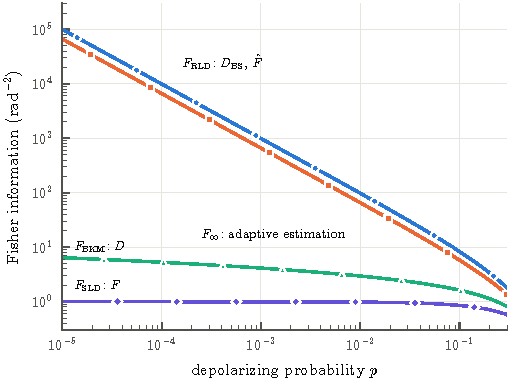
\includegraphics[width=0.6\linewidth]{t4_hierarchy}
\caption{Exact Fisher informations per use at the depolarized qubit gate: $\IR$, which governs $\DBS$ and $\Fg$ and grows as $1/p$; the asymptotic adaptive rate $\Iinf$ of Zhou and Jiang, which grows as $2/(3p)$; $\IB$, which governs the Umegaki divergence and grows as $\frac12\ln(4/p)$; and $\IS$, which governs the Uhlmann fidelity and stays close to one.}
\label{gate:fig:Shier}
\end{figure}

\section{Amplitude damping}\label{gate:sec:ad}

Let $\cA_\gamma$ have Kraus operators $K_0=|0\rangle\langle0|+\sqrt{1-\gamma}|1\rangle\langle1|$ and $K_1=\sqrt\gamma|0\rangle\langle1|$, and write $L_0,L_1$ for those of $\cA_{\gamma'}$. Proofs of the general statements used here are in Example~\ref{cont:ex:amplitude damping}, Section~\ref{chn:sec:ad} and Section~\ref{gate:smp:sec}.

\emph{Infinite converses.} For $\gamma\ne\gamma'$ in $(0,1]$, $\mathrm{ran}J(\cA_\gamma)\cap\mathrm{ran}J(\cA_{\gamma'})=\mathrm{span}\{\vect|0\rangle\langle1|\}$ (the inclusion $\subseteq$, which is all that is used, holds for all $\gamma\ne\gamma'$ in $[0,1]$; Example~\ref{cont:ex:amplitude damping}), and the level decomposition of the pair (Proposition~\ref{chn:prop:adlevels}) has conclusive levels $K_0\cdot K_0^\dagger$ and $L_0\cdot L_0^\dagger$ and a single ambiguous level with operator $S_a=(\gamma+\gamma')|1\rangle\langle1|$. Every $B_s$ entering $\hat C$ is a multiple of $|1\rangle\langle1|$, hence singular, so $\hat Q_s=0$ for all $s\in(0,1)$; hence $\hat C=+\infty$, and $\Fg=\hat Q_{1/2}=0$ gives $-2\ln\Fg=+\infty$. For the barycentric converse~\cite{JMMW2024}, a channel $\mathcal T$ with both BS divergences finite would need $\mathrm{ran}J(\mathcal T)\subseteq\mathrm{span}\{\vect|0\rangle\langle1|\}$, forcing $\mathcal T^*(\Id)\propto|1\rangle\langle1|\ne\Id$; so $C_{\rm bar}=+\infty$. The common kernel vector is $|0\rangle$, on which the two channels act identically.

\emph{Program-simulation converse.} For channels with Kraus operators $(K_k)$ and $(L_l)$, padded to a common length $m$, let
\begin{equation}
\mu_*(\Phi,\Psi)=\max\Big\{|c|:\ \sum_{k,l}C_{lk}L_l^\dagger K_k=c\,\Id,\ \|C\|_\infty\le1\Big\},
\end{equation}
a semidefinite program independent of the Kraus representations. By Theorem~\ref{chn:thm:pureprog} in Chapter~\ref{chn:chapter}, (a) $\mu_*$ is the largest overlap of pure program states from which a single channel $\mathcal L$ simulates both channels, (b) every adaptive strategy with $n$ uses has error probability at least $\frac12(1-\sqrt{1-\mu_*^{2n}})\ge\frac14\mu_*^{2n}$, so $\xi(\Phi,\Psi)\le-2\ln\mu_*$, and (c) no simulation by mixed programs gives a converse below $-\ln\mu_*$. The proof of (b) replaces each use of the unknown channel by $\mathcal L$ acting on a fresh program copy, as in the programmable simulations of Refs.~\cite{PirandolaLupo2017,Pirandola2019}. For amplitude damping the constraint forces $C$ to be diagonal with $C_{00}=c$ and $C_{11}=c(1-a)/\sqrt{\gamma\gamma'}$, $a=\sqrt{(1-\gamma)(1-\gamma')}$, which gives $\mu_*=\sqrt{\gamma\gamma'}/(1-a)$ [Corollary~\ref{chn:cor:adfragile}]. The product input $|1\rangle$ produces the commuting outputs $\mathrm{diag}(\gamma,1-\gamma)$ and $\mathrm{diag}(\gamma',1-\gamma')$, whose classical Chernoff information is a lower bound on $\xi$. With $\Delta=\gamma-\gamma'$,
\begin{equation}
\frac{\Delta^2}{8\gamma(1-\gamma)}+O(\Delta^3)\le\xi(\cA_\gamma,\cA_{\gamma'})\le\frac{\Delta^2}{4\gamma^2(1-\gamma)}+O(\Delta^3).
\end{equation}
The two bounds differ by the factor $2/\gamma$, and simulation arguments cannot close the gap: by Theorem~\ref{chn:thm:pureprog}(c), every program gives at least $-\ln\mu_*$, which exceeds the product-input value by $1/\gamma$ to leading order.

\begin{conjecture*}[Conjecture~\ref{chn:conj:adfid}]%
For every adaptive $n$-use strategy, the fidelity of the two final states is at least $f^{2n}$ with $f=\sqrt{\gamma\gamma'}+\sqrt{(1-\gamma)(1-\gamma')}$. Consequently $\xi(\cA_\gamma,\cA_{\gamma'})\le-2\ln f=\frac{\Delta^2}{4\gamma(1-\gamma)}+O(\Delta^3)$.
\end{conjecture*}

An exact semidefinite program (Uhlmann's theorem~\cite{Uhlmann1976} plus a minimax over $n$-combs) returns $f^n$ for the minimal root fidelity to within $10^{-8}$ for $n\le4$, $\gamma=\frac12$ and $\gamma'\in\{0.05,0.2,0.4,0.47,0.49\}$. The conjecture cannot be proved by amortization: for one pair of different qubit--qubit input states the one-step fidelity ratio is $0.948315<f(\frac12,\frac15)=0.948683$ (40-digit check). The adaptive Fisher information for estimating $\gamma$ is at most $n/(\gamma(1-\gamma))$~\cite{DemkowiczDobrzanskiMaccone2014}, which the product input attains (Remark~\ref{chn:rem:adfisher}); this suggests, but does not prove, that $\xi$ equals the product-input lower bound to leading order. Table~\ref{gate:tab:Sad} lists the values plotted in Fig.~\ref{gate:fig:regimes}(a). Discrimination of amplitude-damping channels with finitely many uses is analyzed in Ref.~\cite{RexitiMancini2021}.

\begin{table}[!tbp]
\centering
\caption{Exponents for $\cA_{1/2}$ against $\cA_{\gamma'}$. The product-input value is a lower bound on $\xi$; $-2\ln\mu_*$ is a proved upper bound and $-2\ln f$ a conjectured one. The single-letter converses $\hat C$, $-2\ln\Fg$ and $C_{\rm bar}$ are infinite in every row.}
\label{gate:tab:Sad}
\begin{tabular}{lccc}
\toprule
$\gamma'$ & product input $|1\rangle$ & $-2\ln f$ (conjectured) & $-2\ln\mu_*$ (proved)\\
\midrule
$0.40$ & $5.077\times10^{-3}$ & $1.015\times10^{-2}$ & $2.252\times10^{-2}$\\
$0.47$ & $4.506\times10^{-4}$ & $9.012\times10^{-4}$ & $1.858\times10^{-3}$\\
$0.49$ & $5.001\times10^{-5}$ & $1.000\times10^{-4}$ & $2.020\times10^{-4}$\\
\bottomrule
\end{tabular}
\end{table}

For replacement channels $\Phi=\Tr(\cdot)\phi$, $\Psi=\Tr(\cdot)\psi$ one has $\mu_*=\FU(\phi,\psi)$, the root fidelity [see the discussion after Theorem~\ref{chn:thm:pureprog}], so $\min\{\hat C,C_{\rm bar},-2\ln\mu_*\}$ is a single-letter converse that does not jump at the pairs of Fig.~\ref{gate:fig:regimes}(b). That example is defined after Theorem~\ref{gate:smp:thm:fragile}; there $\dn{\Phi_t-\Phi}=2\sqrt{t/(1+t)}$, and $\xi=2\ln[(1+t)/(1-t)]=-2\ln\mu_*$ exactly, so the program-simulation converse is tight. Numerically, this value agrees with an independently computed quantum Chernoff bound~\cite{AudenaertChernoff2007} to $1.5\times10^{-8}$, and $-2\ln\FU(\phi_t,\psi_t)$ with $2\ln[(1+t)/(1-t)]$ to $10^{-10}$, while $\Fg\le6\times10^{-16}$ in double precision and $\le8\times10^{-11}$ from the semidefinite program.

\section{The local Stein exponent}\label{gate:sec:local}

\begin{proposition}\label{gate:prop:local}
For the qubit pair $(\cN_{p,\delta},\cN_{p,0})$, $\liminf_{\delta\to0}\zeta/\delta^2\ge\Iinf/2$ and $\limsup_{\delta\to0}\DBS/\zeta\le\IR/\Iinf=(2-p)(3-2p)/(4-3p)<3/2$ for every $p\in(0,1)$.
\end{proposition}

\begin{proof}
Fix $k$ and a parallel $k$-use strategy with an ancilla and input $\rho$. Its outputs $\rho_k^\delta$ have support $\mathrm{supp}(\rho_R)\otimes\mathcal Y^{\otimes k}$ for all $\delta$, because $J(\cN_{p,\delta})\ge\frac p2\Id$ (by the Choi sandwich $(\mathrm{id}\otimes\Psi)(\sigma)\ge\lmin(J(\Psi))\,\sigma_R\otimes\Id$ of Lemma~\ref{shA:lem:sandwichchoi}), and they are analytic in $\delta$. Proposition~\ref{gate:prop:H}(ii) gives $D(\rho_k^\delta\|\rho_k^0)=\frac{\delta^2}{2}F^{\rm BKM}(\rho_k)+O(\delta^3)$, and $F^{\rm BKM}\ge F^{\rm SLD}$. Since $\zeta$ is the regularized (equivalently amortized) channel relative entropy~\cite{WangWilde2019,FFRS2020}, $\zeta\ge\frac1kD(\rho_k^\delta\|\rho_k^0)$. Hence $\liminf_{\delta\to0}\zeta/\delta^2\ge\sup_kF^{\rm SLD}_k/(2k)\ge\Iinf/2$, where $F^{\rm SLD}_k$ is the optimal $k$-use quantum Fisher information and $\Iinf=\lim_kF^{\rm SLD}_k/k$~\cite{ZhouJiang2021}. The upper side is $\zeta\le\DBS=\frac{\delta^2}{2}\IR+O(\delta^4/p^2)$. Finally $(2-p)(3-2p)<\frac32(4-3p)$ is equivalent to $p<\frac54$.
\end{proof}

\emph{Value of $\Iinf$.} With Kraus operators $K_0=\sqrt{1-3p/4}\,\Id$ and $K_j=\sqrt{p/4}\,\sigma_j$, and generator $Z/2$, the span of $\{K_i^\dagger K_j\}$ is all Hermitian matrices, so the Hamiltonian-not-in-Kraus-span condition fails and the scaling is linear~\cite{ZhouJiang2021,DemkowiczDobrzanski2012}. The asymptotic rate is $\Iinf=4\min_{h:\beta(h)=0}\|\alpha(h)\|_\infty$ with $\alpha=(\dot K-ihK)^\dagger(\dot K-ihK)$ and $\beta=iK^\dagger(\dot K-ihK)$~\cite{ZhouJiang2021}. We evaluated a feasible $h$ (upper bound) and the minimax dual with $\rho_0=\Id/2$ (lower bound) in 50-digit arithmetic; they agree to a relative gap below $2\times10^{-47}$ and with
\begin{equation}
\Iinf=\frac{2(1-p)^2}{p(3-2p)},\qquad p\Iinf=\frac23-\frac{8p}{9}+O(p^2),
\end{equation}
which is the closed form of Ref.~\cite[Sec.~VII.A]{ZhouJiang2021} for Pauli noise with $p_x=p_y=p_z=p/4$. A double-precision interior-point solution agrees to $3\times10^{-9}$. Table~\ref{gate:tab:SFinf} lists values.

\begin{table}[!tbp]
\centering
\caption{Asymptotic adaptive Fisher information $\Iinf$ and the RLD information $\IR$ at the depolarized qubit gate, and the resulting bound on $\limsup_{\delta\to0}\DBS/\zeta$.}
\label{gate:tab:SFinf}
\begin{tabular}{lcccc}
\toprule
$p$ & $p\Iinf$ & $p\IR$ & $\IR/\Iinf$ & $p\,\Iinf/2$ (bound on $p\zeta/\delta^2$)\\
\midrule
$10^{-1}$ & 0.578571 & 0.831892 & 1.43784 & 0.289286\\
$10^{-2}$ & 0.657785 & 0.982569 & 1.49375 & 0.328893\\
$10^{-3}$ & 0.665778 & 0.998251 & 1.49938 & 0.332889\\
$10^{-4}$ & 0.666578 & 0.999825 & 1.49994 & 0.333289\\
\bottomrule
\end{tabular}
\end{table}

\begin{conjecture*}[Conjecture~\ref{gate:conj:32}, restated]%
$\lim_{\delta\to0}\DBS/\zeta=\IR/\Iinf$, so that the ratio tends to $3/2$ as $p\to0$.
\end{conjecture*}
The conjecture holds if the local coefficient of $\zeta$ is the SLD rate $\Iinf/2$. A priori it is governed by a relative-entropy (BKM-type) rate, which is at least the SLD rate. For the explicit strategies we evaluated, the BKM rate of a strategy strictly exceeds its own SLD rate, where by the rate of a $k$-use strategy we mean its Fisher information per use, $F_k/k$, which is twice the coefficient of $\delta^2$ in the corresponding divergence per use. For example, the sequential strategy with maximally entangled input has $p\times$(SLD rate) $=0.2334$ but $p\times$(BKM rate) $=0.2992$, i.e., a relative-entropy coefficient $pD_k/(k\delta^2)\to0.1496$. So the limit could lie strictly below $\IR/\Iinf$; all that is established is the bracket $[1,\IR/\Iinf]$. Earlier sequential-strategy bounds, which gave $\DBS/\zeta\le3.34+o(1)$, are superseded by Proposition~\ref{gate:prop:local}.

\section{First-order fragility: task versus bound}\label{gate:sec:m1first}

Theorem~\ref{gate:thm:floor} concerns a \emph{first-order} modulus: the change of a quantity per unit diamond-norm error in the reference channel. This section shows that the adaptive exponents obey the same law as the converses, and that they attain it at the worst case of Theorem~\ref{gate:thm:floor}. The second-order curvature at the pair $(\cN_{p,\delta},\cN_p)$ is a different question; the Chernoff side of it is treated in Sec.~\ref{gate:sec:m1chernoff}.

\emph{Conventions.} In $\zeta(\Phi\|\Psi)$ the channel $\Phi$ is the null hypothesis and $\Psi$ the alternative. The type-I error is that of rejecting $\Phi$, and $\zeta\le\DBS(\Phi\|\Psi)$. Theorem~\ref{gate:thm:floor} perturbs the alternative $\Psi$. For a function $q$ of the reference channel we define the first-order modulus
\begin{equation}\label{gate:eq:m1mod}
\mathrm{Mod}_q(\Psi)=\limsup_{\epsilon\to0}\ \sup_{\dn{\Psi'-\Psi}\le\epsilon}\frac{|q(\Psi')-q(\Psi)|}{\epsilon},
\end{equation}
so that Eq.~\eqref{gate:eq:sharp} reads $\sup_\Phi\mathrm{Mod}_{-2\ln\Fg(\Phi,\cdot)}(\Psi)=1/(2\ltil)$. We write $D_{\max}(\Phi\|\Psi)=\ln\min\{t:J(\Phi)\le tJ(\Psi)\}$. When $J(\Phi)$ is singular, $J(\Psi)\#_0J(\Phi)=J(\Psi)$ by continuity from above, which is why $\hat C$ is defined with the infimum over $s\in(0,1)$; for the rank-one pairs below the infimum is approached as $s\to0$.

\begin{lemma}[CP domination]\label{gate:lem:m1dom}
Suppose $\Psi-c\Phi$ is completely positive for some $c>0$. Then the final states of every $n$-use adaptive strategy satisfy $\rho^{(n)}_\Psi\ge c^n\rho^{(n)}_\Phi$. For every test $T$ with $\alpha_n=\Tr(\Id-T)\rho^{(n)}_\Phi$ and $\beta_n=\Tr T\rho^{(n)}_\Psi$ it follows that $\beta_n\ge c^n(1-\alpha_n)$ and $\frac12(\alpha_n+\beta_n)\ge\frac12c^n$. In particular $\zeta(\Phi\|\Psi)\le D_{\max}(\Phi\|\Psi)$ and $\xi(\Phi,\Psi)\le D_{\max}(\Phi\|\Psi)$.
\end{lemma}

\begin{proof}
The final state is a composition of completely positive maps, each use of the channel contributing a factor $\Psi\otimes\mathrm{id}$. Writing $\Psi=c\Phi+(\Psi-c\Phi)$ in every slot and expanding, all $2^n$ terms are positive semidefinite, and one of them is $c^n\rho^{(n)}_\Phi$. The best constant is $c=e^{-D_{\max}(\Phi\|\Psi)}$.
\end{proof}

\begin{proposition}[Thompson--Lipschitz property]\label{gate:prop:m1thompson}
Let $\Phi,\Psi,\Psi'$ be channels with $J(\Psi)>0$. Each of $\zeta(\Phi\|\cdot)$, $\xi(\Phi,\cdot)$, $\DBS(\Phi\|\cdot)$, $\hat C(\Phi,\cdot)$, $-2\ln\Fg(\Phi,\cdot)$, $D(\Phi\|\cdot)$ and $-2\ln \FU(\Phi,\cdot)$ changes by at most $d_T(\Psi,\Psi')$ when $\Psi$ is replaced by $\Psi'$. By Eq.~\eqref{gate:eq:Ssandwich}, each has $\mathrm{Mod}\le1/(2\ltil(\Psi))$.
\end{proposition}

\begin{proof}
Let $t=d_T(\Psi,\Psi')$.

\emph{Operational exponents.} For $\zeta$ this is Theorem~\ref{shA:thm:thompson} in Chapter~\ref{shA:chapter}; the following argument also covers $\xi$. Since $e^t\Psi-\Psi'$ is completely positive, the expansion in Lemma~\ref{gate:lem:m1dom} gives $\rho^{(n)}_{\Psi'}\le e^{nt}\rho^{(n)}_\Psi$ for the same strategy. Hence $\beta_n$ and the Bayes error grow by at most $e^{nt}$, so $\zeta(\Phi\|\Psi')\ge\zeta(\Phi\|\Psi)-t$ and $\xi(\Phi,\Psi')\ge\xi(\Phi,\Psi)-t$. Exchanging $\Psi$ and $\Psi'$ gives the other direction.

\emph{The BS divergence.} From $J(\Psi')^{-1}\ge e^{-t}J(\Psi)^{-1}$ and operator monotonicity of $\ln$ on the support of $J_\Phi^{1/2}J_\Psi^{-1}J_\Phi^{1/2}$, which equals the support of $J_\Phi$, we get $J_\Phi^{1/2}\ln(\cdot)J_\Phi^{1/2}\ge(\text{same at }\Psi)-tJ_\Phi$. Moreover $\Tr_{\mathcal Y}J_\Phi=\Id$.

\emph{The remaining quantities.} $\hat C$ and $\Fg$ follow as in the proof of Theorem~\ref{gate:thm:floor}. $D$ and $\FU$ follow from monotonicity of $\ln$ and of the fidelity in each argument.
\end{proof}

Thus every quantity considered, operational or not, is 1-Lipschitz in the relative (Thompson) error. The factor $1/\ltil$ arises only when a diamond-norm error is converted into a relative one, through Lemma~\ref{gate:lem:J}.

\begin{proposition}[The worst case of Theorem~\ref{gate:thm:floor} is genuinely fragile]\label{gate:prop:m1worst}
Let $d_X=d_Y=d$ and let $\Psi$ be a channel with $J(\Psi)>0$. Let $W$ be unitary with $J(\Psi)v_W=\mu v_W$ for $v_W=\vect W$, and put $\tilde\mu=\mu/d$, $\hat v_W=v_W/\sqrt d$ and $\sigma=J(\Psi)/d$.
\begin{enumerate}
\item[(a)] The exponents, converses and comparison quantities all coincide:
\begin{equation*}
\begin{split}
&\zeta(\mathrm{Ad}_W\|\Psi)=\xi(\mathrm{Ad}_W,\Psi)=D(\mathrm{Ad}_W\|\Psi)=\DBS(\mathrm{Ad}_W\|\Psi)\\
&\quad=\hat C(\mathrm{Ad}_W,\Psi)=-2\ln\Fg(\mathrm{Ad}_W,\Psi)=-2\ln\FU(\mathrm{Ad}_W,\Psi)=\ln(1/\tilde\mu).
\end{split}
\end{equation*}
\item[(b)] Let $\mathcal M$ be Hermitian preserving and trace annihilating. Along $\Psi+e\mathcal M$, each quantity in (a) is differentiable at $e=0$ with the common derivative $-\langle\hat v_W,J(\mathcal M)\hat v_W\rangle/\mu$. Each is in fact Fr\'echet differentiable at $\Psi$.
\item[(c)] Each quantity in (a) has $\mathrm{Mod}=1/(2\tilde\mu)$, attained by $\mathcal M=\frac12(\mathrm{Ad}_W-\mathrm{Ad}_{W'})$ with $\Tr W^\dagger W'=0$. If $\mu=\lambda(\Psi)$, as at the worst case of Theorem~\ref{gate:thm:floor}, this equals $1/(2\ltil)$, the bound of Proposition~\ref{gate:prop:m1thompson}.
\item[(d)] For $\Psi=\mathcal P_q\circ\mathrm{Ad}_U$ and $W=QU$, statement (a) holds at every Pauli channel $\mathcal P_{q'}\circ\mathrm{Ad}_U$ with $\tilde\mu=q'_Q$. Along the direction in (c), every quantity equals $\ln[1/(q_Q+e/2)]$ exactly.
\end{enumerate}
\end{proposition}

\begin{proof}
(a) \emph{Upper bound.} $J(\Psi)-c\,v_Wv_W^\dagger\ge0$ holds if and only if $c\le1/\langle v_W,J(\Psi)^{-1}v_W\rangle=\tilde\mu$. Lemma~\ref{gate:lem:m1dom} with $c=\tilde\mu$ then gives $\zeta,\xi\le\ln(1/\tilde\mu)$.

\emph{Lower bound.} Use the maximally entangled input and the test $\{\hat v_W\hat v_W^\dagger,\Id-\hat v_W\hat v_W^\dagger\}$, accepting $\mathrm{Ad}_W$ only if all $n$ outcomes are $\hat v_W$. This gives $\alpha_n=0$ and $\beta_n=\langle\hat v_W,\sigma\hat v_W\rangle^n=\tilde\mu^n$. For a Pauli channel the test is the Bell measurement in the known frame.

\emph{Converses.} For rank-one $J_\Phi=v_Wv_W^\dagger$ and any $J>0$ we have $J_\Phi^{1/2}\ln(J_\Phi^{1/2}J^{-1}J_\Phi^{1/2})J_\Phi^{1/2}=\ln\langle v_W,J^{-1}v_W\rangle\,v_Wv_W^\dagger$ and $J\#_sv_Wv_W^\dagger=\langle v_W,J^{-1}v_W\rangle^{s-1}v_Wv_W^\dagger$ for $s\in(0,1]$. Moreover $\Tr_{\mathcal Y}v_Wv_W^\dagger=\Id$. Hence $\DBS=\hat C=-2\ln\Fg=D_{\max}=\ln\langle v_W,J^{-1}v_W\rangle$, which equals $\ln(1/\tilde\mu)$.

\emph{Umegaki and Uhlmann.} $\ln(1/\tilde\mu)=-\langle\hat v_W,\ln\sigma\,\hat v_W\rangle\le D\le D_{\max}$. Also $\tilde\mu\le\FU^2\le\langle\hat v_W,\sigma\hat v_W\rangle=\tilde\mu$, where the first inequality is domination and the second uses the maximally entangled input.

(b) Put $u(e)=\ln\langle\hat v_W,\sigma_e^{-1}\hat v_W\rangle$, $\ell_1(e)=-\langle\hat v_W,\ln\sigma_e\,\hat v_W\rangle$ and $\ell_2(e)=-\ln\langle\hat v_W,\sigma_e\hat v_W\rangle$. The arguments of (a) hold at every $\Psi_e$, and give $\ell_1\le D,\zeta\le u$ and $\ell_2\le\xi,-2\ln\FU\le u$. The first four quantities of (a) are equal to $u$ for all $e$. The three bounding functions are smooth and coincide at $e=0$. Because $\hat v_W$ is an eigenvector of $\sigma$, their derivatives also coincide there and equal $-\langle\hat v_W,J(\mathcal M)\hat v_W\rangle/(d\tilde\mu)$.

(c) By Lemma~\ref{gate:lem:J}, $|\langle\hat v_W,J(\mathcal M)\hat v_W\rangle|\le\frac d2\dn{\mathcal M}$. For the stated $\mathcal M$ the left side equals $d/2$ and $\dn{\mathcal M}=1$.

(d) The vector $\vect(QU)$ is an eigenvector of $J(\mathcal P_{q'}\circ\mathrm{Ad}_U)$ with eigenvalue $dq'_Q$.
\end{proof}

\begin{remark}\label{gate:rem:m1hier}
At this worst case the Umegaki divergence and the Uhlmann fidelity also equal $\ln(1/\ltil)$ and move at the rate $1/(2\ltil)$. The worst direction changes a floor eigenvalue, and by Proposition~\ref{gate:prop:H}(iv) such incoherent perturbations do not separate the metrics. The hierarchy RLD ($\sim1/\ltil$), BKM ($\sim\ln(1/\ltil)$) and SLD ($O(1)$) is therefore a statement about second-order curvature under coherent errors. It does not hold per unit of diamond distance.
\end{remark}

For a general unitary $\Phi=\mathrm{Ad}_W$ the same arguments give a sandwich:
\begin{equation}\label{gate:eq:m1sandwich}
-\ln\langle\hat v_W,\sigma\hat v_W\rangle\le\xi\le\zeta\le\DBS=\hat C=-2\ln\Fg=\ln\langle\hat v_W,\sigma^{-1}\hat v_W\rangle,\qquad\zeta\ge-\langle\hat v_W,\ln\sigma\,\hat v_W\rangle.
\end{equation}
By Jensen's inequality, its two ends coincide if and only if $\hat v_W$ is an eigenvector of $\sigma$.

\begin{lemma}[Tight converses pass on their sensitivity]\label{gate:lem:m1tight}
Let $f\le g$ near $\Psi$, with $J(\Psi)>0$ and $f(\Psi)=g(\Psi)$, and let $g$ be Fr\'echet differentiable at $\Psi$. Then $\mathrm{Mod}_f(\Psi)\ge\mathrm{Mod}_g(\Psi)$. If $g$ is only directionally differentiable, then $\mathrm{Mod}_f\ge\sup_{\dn{\mathcal M}=1}\max\{0,-g'(\Psi;\mathcal M)\}$.
\end{lemma}

\begin{proof}
Choose $\mathcal M$ with $\dn{\mathcal M}=1$ along which $g$ decreases, $g'(\Psi;\mathcal M)=-c\le0$. Then $f(\Psi+e\mathcal M)\le g(\Psi+e\mathcal M)=f(\Psi)-ce+o(e)$, so $|f(\Psi+e\mathcal M)-f(\Psi)|\ge ce-o(e)$.
\end{proof}

Applied with $f\in\{\zeta,\xi\}$ and $g$ a converse, the lemma shows two things. First, wherever a converse is tight, the exponent is at least as sensitive at first order as the converse. Second, by Proposition~\ref{gate:prop:m1thompson}, the exponent is never more sensitive than $1/(2\ltil)$. A first-order spurious gap can therefore occur only at pairs where the converse already overestimates the exponent, that is, at pairs that are spurious at zeroth order.

\begin{proposition}[Pauli-diagonal pairs]\label{gate:prop:m1pauli}
Let $\Phi=\mathcal P_a\circ\mathrm{Ad}_U$ and $\Psi=\mathcal P_b\circ\mathrm{Ad}_U$ with all $b_Q>0$. Then $\zeta(\Phi\|\Psi)=D(\Phi\|\Psi)=\DBS(\Phi\|\Psi)=\sum_Qa_Q\ln(a_Q/b_Q)$, $\xi(\Phi,\Psi)=\hat C(\Phi,\Psi)=-\ln\inf_{s\in(0,1)}\sum_Qa_Q^sb_Q^{1-s}$, and $\Fg=\sum_Q\sqrt{a_Qb_Q}$.
\end{proposition}

\begin{proof}
\emph{Achievability.} The Bell measurement in the known frame produces i.i.d.\ samples of $a$ or of $b$, to which the classical Stein and Chernoff theorems apply.

\emph{Converse.} As in the proof of Proposition~\ref{gate:prop:N34}(a), the final state of any strategy is $\Lambda(a^{\otimes n})$ or $\Lambda(b^{\otimes n})$ for a channel $\Lambda$ independent of the rates. Any test therefore pulls back to a test between i.i.d.\ classical sources.

\emph{Values of the converses.} The two Choi matrices commute, and $\Tr_{\mathcal Y}$ of each projector onto $\vect(QU)$ is $\Id$.
\end{proof}

On this class the single-letter converses are exact, so their sensitivity along Pauli directions belongs to the task at every order. The pair $(\cN_{p,\delta},\cN_p)$ is not in this class, because the miscalibration is coherent.

\begin{proposition}[A first-order spurious gap]\label{gate:prop:m1gap}
Take preparation channels ($d_X=1$, so $\ltil=\lambda$ and the diamond norm is the trace norm). Let $\sigma=\mathrm{diag}(1-\lambda,\lambda)$ and $\phi=\sqrt{1-y\lambda}\,|0\rangle+\sqrt{y\lambda}\,|1\rangle$ with $0<y<1/\lambda$.
\begin{enumerate}
\item[(a)] The converses are $\DBS=\hat C=-2\ln\Fg=\ln[(1-y\lambda)/(1-\lambda)+y]$, which tends to $\ln(1+y)$.
\item[(b)] The exponents are $\zeta=-(1-y\lambda)\ln(1-\lambda)-y\lambda\ln\lambda$ and $\xi=-\ln[(1-y\lambda)(1-\lambda)+y\lambda^2]$.
\item[(c)] The first-order moduli are
\begin{equation}\label{gate:eq:m1gap}
\begin{gathered}
\mathrm{Mod}_{\DBS}=\frac{y}{2(1+y)\lambda}[1+O(\lambda)],\\
\mathrm{Mod}_\zeta=\tfrac12|1-y|+O(\lambda\ln^2\tfrac1\lambda)\ (y\neq1),\qquad \mathrm{Mod}_\xi=\tfrac12+O(\lambda),
\end{gathered}
\end{equation}
and at $y=1$, $\mathrm{Mod}_\zeta=\sqrt{\lambda(1-\lambda)}\ln[(1-\lambda)/\lambda]/(1-2\lambda)$.
\end{enumerate}
\end{proposition}

\begin{proof}
\emph{Exponents.} The quantum Stein lemma gives $\zeta=D(\phi\|\sigma)$. For pure $\phi$ the quantity $\langle\phi,\sigma^t\phi\rangle$ is minimized over $t\in[0,1]$ at $t=1$, which gives $\xi$.

\emph{Moduli.} For traceless $\mathcal M$ with $\|\mathcal M\|_1\le1$, $\sup|\Tr\mathcal M H|=\frac12[\lmax(H)-\lmin(H)]$. The derivative operators are $H=vv^\dagger/\langle\phi,\sigma^{-1}\phi\rangle$ with $v=\sigma^{-1}\phi$ for the converse, the Hadamard product of $\phi\phi^\dagger$ with the divided differences of $\ln$ for $D$, and $\phi\phi^\dagger/\langle\phi,\sigma\phi\rangle$ for $\xi$.
\end{proof}

The ratio $\mathrm{Mod}_{\DBS}/\mathrm{Mod}_\zeta$ is of order $1/\lambda$; at $y=1$ the two moduli are $1/(4\lambda)$ and roughly $\sqrt\lambda\ln(1/\lambda)$. The values already differ at zeroth order, as Lemma~\ref{gate:lem:m1tight} requires. For replacement channels on a qubit, every adaptive strategy outputs $\Lambda(\phi^{\otimes n})$ or $\Lambda(\sigma'^{\otimes n})$, so the same moduli hold along replacement directions.

\emph{The slope maximizer of Proposition~\ref{gate:prop:L2}.} Let $\Phi=\mathrm{Ad}_{R_Z(\theta)U}$ and $\Psi=\Dp\circ\mathrm{Ad}_U$ with $\sin^2(\theta/2)=p/2$, the unitary that maximizes the absolute slope of $\Fg$. Here $\Fg\to1/\sqrt3$, and all converses equal $\ln[(1-p/2)/(1-3p/4)+2]\to\ln3$. Table~\ref{gate:tab:m1L2} brackets $\zeta$. The lower bound comes from sequential strategies with maximally entangled input. The upper bound is the one-copy divergence $D^\#_\alpha$ of Ref.~\cite{FawziFawzi2021}, re-checked and rescaled in 40-digit arithmetic. The converse overshoots $\zeta$ by a certified factor that grows as $p$ decreases. The absolute slope $0.3849/p$ of Proposition~\ref{gate:prop:L2} is therefore a slope of the converse at a pair where the converse is already spurious. The first-order modulus of $\zeta$ at this pair is not determined.

\begin{table}[!tbp]
\centering
\caption{Converse and Stein exponent at the slope maximizer of Proposition~\ref{gate:prop:L2}. The integer $k$ is the number of sequential uses in the best lower-bound strategy. $U_3$ is Eq.~\eqref{gate:eq:Sstein} at the base pair $(\mathrm{Ad}_U,\Psi)$, where $\zeta=-\ln(1-3p/4)$ by Proposition~\ref{gate:prop:m1worst}.}
\label{gate:tab:m1L2}
\begin{tabular}{lcccccc}
\toprule
$p$ & $\DBS=-2\ln\Fg$ & $\zeta\ge$ ($k$) & $\zeta\le D^\#_\alpha$ ($1/\alpha$) & $\zeta\le U_3$ & ratio $\ge$ & ratio $\le$\\
\midrule
$10^{-2}$ & 1.09945 & 0.17298 (14) & 0.48014 (11/16) & 0.78916 & 2.29 & 6.36\\
$10^{-3}$ & 1.09870 & 0.071789 (46) & 0.22020 (3/4) & 0.32478 & 4.99 & 15.3\\
$10^{-4}$ & 1.09862 & 0.028417 (151) & 0.091412 (3/4) & 0.12692 & 12.0 & 38.7\\
\bottomrule
\end{tabular}
\end{table}

\emph{Numerical checks.} All entries below were computed from direct $4\times4$ and $16\times16$ matrices in 40-digit arithmetic, without using the closed forms.
\begin{itemize}
\item \emph{Proposition~\ref{gate:prop:m1worst}(a).} Cases: depolarizing noise with $p=10^{-2},10^{-3},10^{-4}$; a biased Pauli channel ($q_Z=10^{-3}$, $q_X=q_Y=10^{-5}$) with $W$ chosen both on and off the floor; and two qubits with $U=\mathrm{CNOT}$ and $W=(Z\otimes X)U$. In every case $-2\ln\Fg$, $\DBS$, $D_{\max}$, the Umegaki divergence at maximally entangled input, the Bell-test exponent and $-2\ln\FU$ equal $\ln(1/q_W)$ to $10^{-24}$ or better. $\hat C$ agrees to $10^{-12}$, because its infimum is approached only as $s\to0$.
\item \emph{Proposition~\ref{gate:prop:m1worst}(b).} In the direction of Theorem~\ref{gate:thm:floor} and in three random directions per case, the derivatives of $u$, $\DBS$, $\ell_1$ and $\ell_2$ agree with $-\langle\hat v_W,J(\mathcal M)\hat v_W\rangle/\mu$ to $3\times10^{-16}$. In that direction the slope times $2q_W$ is $1$.
\item \emph{Proposition~\ref{gate:prop:m1thompson}.} Over eight random pairs, the largest ratio $|\mathcal M q|/d_T$ is $0.74$.
\item \emph{Proposition~\ref{gate:prop:m1pauli}.} The deviations are at most $2\times10^{-40}$ ($\DBS$) and $3\times10^{-16}$ ($\hat Q_s$).
\item \emph{Proposition~\ref{gate:prop:m1gap}.} The moduli agree with finite-difference suprema to all printed digits.
\end{itemize}

\section{The Chernoff exponent at a noisy gate}\label{gate:sec:m1chernoff}

For the pair of Sec.~\ref{gate:sec:local}, Theorem~\ref{gate:thm:B} gives the exact value
\begin{equation}\label{gate:eq:m1C}
\hat C(\cN_{p,\delta},\cN_p)=-\ln\Big[\frac p2+\Big(1-\frac p2\Big)(1+x)^{-1/2}\Big]=\frac{\IR}{8}\delta^2+O(\delta^4/p^2),
\end{equation}
with $x=4(1-p)^2\sin^2(\delta/2)/[p(4-3p)]$. We compare it with $\xi$.

\begin{lemma}[Midpoint bound]\label{gate:lem:m1mid}
Call $B$ a strong-converse Stein bound if every $n$-use adaptive strategy and test $T$ satisfy $\Tr T\rho^{(n)}_\Psi\ge c(\Tr T\rho^{(n)}_\Gamma)\,e^{-nB(\Gamma\|\Psi)-o(n)}$, for some function $c$ with $c(t)>0$ whenever $t>0$. For such a $B$ and any channels $\Phi,\Psi,\Gamma$,
\begin{equation}
\xi(\Phi,\Psi)\le\max\{B(\Gamma\|\Phi),B(\Gamma\|\Psi)\}.
\end{equation}
The following are strong-converse Stein bounds:
\begin{itemize}
\item $D_{\max}$, by Lemma~\ref{gate:lem:m1dom};
\item the geometric R\'enyi divergences $\hat D_\alpha$ with $\alpha\in(1,2]$, by their chain rule~\cite{FangFawzi2021} together with $\tilde D_\alpha\le\hat D_\alpha$ and
\begin{equation*}
\Tr T\sigma\ge(\Tr T\rho)^{\alpha/(\alpha-1)}e^{-\tilde D_\alpha(\rho\|\sigma)};
\end{equation*} letting $\alpha\downarrow1$ gives $\DBS$;
\item the one-copy $D^\#_\alpha$~\cite{FawziFawzi2021}.
\end{itemize}
At the gate, $\xi(\cN_{p,\delta},\cN_p)\le B(\cN_{p,\delta/2}\|\cN_p)$.
\end{lemma}

\begin{proof}
Let $T$ be the decision ``$\Phi$''. Whether $\Tr T\rho_\Gamma\ge\frac12$ or $\Tr(\Id-T)\rho_\Gamma>\frac12$, one of the two error terms is at least $\frac12c(\frac12)e^{-nB-o(n)}$. At the gate take $\Gamma=\cN_{p,\delta/2}$. Post-rotation by $R_Z(-\delta/2)$, and conjugation by $X$ combined with a rotation, show that $B(\Gamma\|\cN_{p,\delta})=B(\Gamma\|\cN_p)$.
\end{proof}

The two-copy bound $\frac12D^\#_\alpha(\cN^{\otimes2}\|\cN_0^{\otimes2})$ used for $\zeta_+$ is not included in the list, because it bounds $\zeta$ only through $\zeta=D^{\rm reg}$, which is a weak converse.

\begin{proposition}[Local Chernoff exponent]\label{gate:prop:m1local}
For every $p\in(0,1)$,
\begin{equation}\label{gate:eq:m1local}
\frac{\Iinf}{8}=\frac{(1-p)^2}{4p(3-2p)}\le\liminf_{\delta\to0}\frac{\xi}{\delta^2}\le\limsup_{\delta\to0}\frac{\xi}{\delta^2}\le\frac{\IR}{8}=\frac{(1-p)^2(2-p)}{4p(4-3p)}.
\end{equation}
Hence $1\le\liminf_{\delta\to0}\hat C/\xi\le\limsup_{\delta\to0}\hat C/\xi\le\IR/\Iinf=(2-p)(3-2p)/(4-3p)<3/2$, the same bracket as for $\DBS/\zeta$. As $p\to0$, $p\,\xi/\delta^2\in[\frac1{12},\frac18]$.
\end{proposition}

\begin{proof}
\emph{Upper bound.} Use $\xi\le\hat C$ (Theorem~\ref{chn:thm:main}). Alternatively, Lemma~\ref{gate:lem:m1mid} with $B=\DBS$ gives $\xi\le\DBS(\cN_{p,\delta/2}\|\cN_p)=\frac{\IR}{2}(\frac\delta2)^2+O(\delta^4/p^2)$, which has the same constant and uses only Ref.~\cite{FangFawzi2021}.

\emph{Lower bound.} The argument follows Proposition~\ref{gate:prop:local}. Fix $k$ and a parallel $k$-use strategy with an ancilla. Its outputs $\rho_k^\delta$ have $\delta$-independent support and are analytic in $\delta$. The quantum Chernoff theorem~\cite{AudenaertChernoff2007,NussbaumSzkola2009}, applied to i.i.d.\ blocks, gives $\xi\ge\frac1kC(\rho_k^\delta,\rho_k^0)$. Moreover $C\ge-\ln\Tr\sqrt{\rho_k^\delta}\sqrt{\rho_k^0}\ge-\ln\FU\ge1-\FU=\frac{\delta^2}{8}F^{\rm SLD}(\rho_k)+O(\delta^3)$ by Proposition~\ref{gate:prop:H}(ii). Taking the supremum over $k$ and using Ref.~\cite{ZhouJiang2021} gives $\Iinf/8$.
\end{proof}

The lower-bound argument discards a Wigner--Yanase factor: a fixed strategy has local coefficient $F^{\rm WY}(\rho_k)/(8k)$, with $F^{\rm SLD}\le F^{\rm WY}\le2F^{\rm SLD}$. For the sequential strategy below, the Chernoff constant exceeds that strategy's own SLD rate by a factor $1.186$. The exact local constant within Eq.~\eqref{gate:eq:m1local} is therefore open, as it is for $\zeta$ (Conjecture~\ref{gate:conj:32}).

\emph{Explicit strategies.} Each formula below was verified against explicit simulation for $k\le3$ to 20 digits. We consider three strategies.
\begin{itemize}
\item \emph{(P) Bell measurement after each use.} This gives the classical Chernoff information of $(q_I,q_Z,\frac p2)$ against $(q_Ic^2+q_Zs^2,\,q_Zc^2+q_Is^2,\,\frac p2)$ with $s=\sin\frac\delta2$, which is of order $\delta^4/p$.
\item \emph{(A) $k$ sequential uses on half of a Bell pair}, with $U^\dagger$ between uses and a collective measurement on i.i.d.\ blocks:
\begin{equation}
\xi\ge-\frac1k\ln\Big[1-\sin^2\frac{k\delta}{2}\Big(\sqrt{1-\tfrac{3q_k}{4}}-\sqrt{\tfrac{q_k}{4}}\Big)^2\Big],\qquad q_k=1-(1-p)^k .
\end{equation}
\item \emph{(B) The heralded code of Sec.~\ref{gate:sec:finite}}, with abort on a flag, $r_k=(1-2a)^k$ and $a=(p/4)/(1-p/2)$:
\begin{equation}
\xi\ge-\frac1k\ln\Big[1-\big(1-\tfrac p2\big)^k\big(1-\sqrt{1-r_k^2}\big)\sin^2\frac{k\delta}{2}\Big].
\end{equation}
\end{itemize}
For (A) with $k=1$, i.e.\ a product strategy with a collective measurement, $p\,\xi/\delta^2\to p/4\to0$. Single-use strategies therefore have curvature of order one, and the $1/p$ curvature is produced by adaptive accumulation. As $p\to0$, the local constants of (A) and (B) tend to
\begin{equation}
\begin{gathered}
c_A=\max_u\frac u{16}\Big(\sqrt{4-3(1-e^{-u})}-\sqrt{1-e^{-u}}\Big)^2=0.0345901,\\
c_B=\max_u\frac u4e^{-u/2}\Big(1-\sqrt{1-e^{-u}}\Big)=0.0365266 .
\end{gathered}
\end{equation}
Table~\ref{gate:tab:m1local} lists their finite-$p$ values.

\begin{table}[!tbp]
\centering
\caption{Local constants $p\,\xi/\delta^2$ as $\delta\to0$, maximized over the number $k$ of sequential uses (in parentheses). The entry $p\IR/8$ equals $p\hat C/\delta^2$.}
\label{gate:tab:m1local}
\begin{tabular}{lccccc}
\toprule
$p$ & (A) & (B) & $p\Iinf/8$ & $p\IR/8$ & product ($k=1$)\\
\midrule
$10^{-2}$ & 0.034417 (51) & 0.036303 (57) & 0.082223 & 0.122821 & 0.00224\\
$10^{-3}$ & 0.034573 (514) & 0.036504 (568) & 0.083222 & 0.124781 & 0.000242\\
$10^{-4}$ & 0.034588 (5145) & 0.036524 (5684) & 0.083322 & 0.124978 & 0.0000247\\
$\to0$ & 0.0345901 & 0.0365266 & $1/12$ & $1/8$ & 0\\
\bottomrule
\end{tabular}
\end{table}

\begin{proposition}[Finite miscalibration]\label{gate:prop:m1finite}
(a) For $p\ll\delta\ll1$, strategy (A) with $k=\lfloor\pi/\delta\rfloor$ gives $\xi\ge\frac{\delta}{2\pi}\ln\frac{\delta}{\pi p}\,[1+o(1)]$.
(b) By Eq.~\eqref{gate:eq:Sstein} (Corollary~\ref{shA:cor:stein}), $\xi\le\zeta\le U_3=\frac\delta2[\ln\frac4p+\ln\frac2\delta+O(1)]$, and since $\hat C(c\sqrt p)\to\frac12\ln(1+c^2/4)$,
\begin{equation}
\sup_\delta\frac{\hat C}{\xi}\ge\frac{0.2682+o(1)}{\sqrt p\,\ln(1/p)},\qquad 0.2682=\max_c\frac{\ln(1+c^2/4)}{1.5\,c}.
\end{equation}
\end{proposition}

\begin{proof}
(a) With $k\delta\simeq\pi$ the block Chernoff bound is $-\ln[q_k/2+2\sqrt{(1-\tfrac{3q_k}{4})\tfrac{q_k}{4}}]=\frac12\ln\frac1{q_k}[1+o(1)]$, where $q_k\simeq\pi p/\delta$. Dividing by $k\simeq\pi/\delta$ gives the claim.
(b) Expand $U_3$ with $\epsilon'=(1-p)\sin(\delta/2)$ and use $h(\epsilon')=\epsilon'\ln(1/\epsilon')+O(\epsilon')$. At $\delta=c\sqrt p$ this gives $U_3=\frac\delta2[\frac32\ln\frac1p+O(1)]$; maximize over $c$.
\end{proof}

The curvature of $\hat C$ is thus genuine for $\delta\lesssim p\ln(1/p)$ and spurious for $p\ln(1/p)\lesssim\delta\lesssim\sqrt p$. In the latter range $\xi$ grows only linearly in $\delta$ (up to logarithms), while $\hat C$ keeps its $\delta^2/(8p)$ curvature. These are the same three scales as for the Stein exponent.

Table~\ref{gate:tab:m1cross} gives certified numbers. The upper bound is $\xi_+=\min\{\hat C(\delta),B(\delta/2)\}$, where $B$ is the smallest of $\DBS$, the certified one-copy $D^\#_\alpha$ of Sec.~\ref{gate:sec:finite}, $D_{\max}=2\operatorname{arsinh}\sqrt{x}$ and $\ln(4/p)$. The lower bound $\xi_-$ is the best of (P), (A) and (B). Above the onset the binding upper bound is $D^\#_\alpha$ at $\delta/2$, so the certified overshoot rests on Refs.~\cite{FangFawzi2021,FawziFawzi2021} and Lemma~\ref{gate:lem:m1mid} only. The bound~\eqref{gate:eq:Sstein} is never binding. The program-simulation converse of Theorem~\ref{chn:thm:pureprog} gives $-2\ln\mu_*\ge1.34\,\hat C$ at every tested point, so it does not help at this pair.

\begin{table}[!tbp]
\centering
\caption{Chernoff exponent at finite $\delta$, with $x=\delta/(p\ln(1/p))$. Ratios divided by $\xi_+$ are certified lower bounds on $\hat C/\xi$; ratios divided by $\xi_-$ are upper bounds.}
\label{gate:tab:m1cross}
\small
\begin{tabular}{lccc}
\toprule
 & $p=10^{-2}$ & $p=10^{-3}$ & $p=10^{-4}$\\
\midrule
small-$x$ value of $\hat C/\xi_-$ ($x=0.02$) & 3.38 & 3.42 & 3.42\\
smallest $x$ with $\hat C/\xi_+>1.01$ & 3.17 & 1.59 & 1.26\\
maximum of $\hat C/\xi_+$ & 1.125 ($\delta=0.29$) & 2.483 ($\delta=0.087$) & 5.996 ($\delta=0.029$)\\
peak of $\hat C/\xi_+$ times $\sqrt p\ln(1/p)$ & 0.52 & 0.54 & 0.55\\
maximum of $\hat C/\xi_-$ & 5.23 & 11.1 & 26.4\\
$\xi_+/\xi_-$ over the grid & 1.05--4.95 & 2.36--5.30 & 3.42--5.29\\
\bottomrule
\end{tabular}
\end{table}

\section{The Stein exponent at finite miscalibration}\label{gate:sec:finite}

\emph{Lower bounds.} Each lower bound is $\zeta\ge D_k/k$ for an explicit $k$-use strategy, maximized over integer $k\le\max(10/p,50/\delta)$. (A) Sequential, maximally entangled input, $U^\dagger$ between uses: $D_k=(1-q)\sin^2(k\delta/2)\ln[1+4(1-q)/q]$ with $q=1-(1-p)^k$. (B) Sequential with a heralded two-qubit code $\{|00\rangle,|11\rangle\}$ (probe plus noiseless ancilla), in which bit-flip errors are flagged and phase errors act as logical dephasing: $D_k=(1-\frac p2)^k\,c_k\operatorname{artanh}(c_k)\,(1-\cos k\delta)$ with $c_k=(1-2a)^k$, $a=(p/4)/(1-p/2)$. Both formulas were verified by explicit simulation for $k\le3$ to 20 digits. As $\delta/p\to0$ they give $p\zeta/\delta^2\ge0.149587$ (A) and $0.158119$ (B). These finite-length strategies fall short of the asymptotic coefficient $p\Iinf/2\to1/3$ of Proposition~\ref{gate:prop:local}, which is why the small-$\delta$ ratio $\DBS/\zeta_-\approx0.5/0.158=3.16$ in Fig.~\ref{gate:fig:crossover}(a) lies above the proved bracket $[1,\IR/\Iinf]$: the numerical bracket for $\bar\delta\lesssim1$ is $[1,3.16]$, and only in the limit $\delta\to0$ does Proposition~\ref{gate:prop:local} narrow it to $[1,\IR/\Iinf]\subset[1,3/2]$.

\emph{Upper bounds.} $\zeta_+=\min\{\DBS,\ U_3,\ \ln(4/p),\ D^\#_\alpha,\ \frac12D^\#_\alpha(\cN^{\otimes2}\|\cN_0^{\otimes2})\}$. Here $U_3$ is Eq.~\eqref{gate:eq:Sstein} applied at the pair $(\cN_{p,0},\cN_{p,0})$, where $\zeta=0$ and $d_T=0$, with $\epsilon'=(1-p)|\sin(\delta/2)|$ (checked against the diamond-norm semidefinite program) and $\kappa=(4-3p)/p$. The Fawzi--Fawzi divergences satisfy $\zeta\le\widetilde D^{\rm reg}_\alpha\le D^\#_\alpha$ for $\alpha>1$~\cite{FawziFawzi2021}; we solved their semidefinite programs for $1/\alpha$ on a dyadic grid in $[\frac12,\frac{31}{32}]$, re-checked each solution in 25-digit arithmetic and rescaled it to be exactly feasible, so each value is a valid upper bound. The two-copy program was solved on alternate grid points; it improved $\zeta_+$ by up to $6.8\%$ at $p=10^{-2}$ and by at most $0.5\%$ at $p=10^{-3}$.

\begin{table}[!tbp]
\centering
\caption{Key numbers of Fig.~\ref{gate:fig:crossover} and Fig.~\ref{gate:fig:Sfid}, with $\bar\delta=\delta/(p\ln(1/p))$. Ratios divided by $\zeta_+$ are certified lower bounds on the true ratio; ratios divided by $\zeta_-$ are upper bounds.}
\label{gate:tab:Scross}
\begin{tabular}{lccc}
\toprule
 & $p=10^{-2}$ & $p=10^{-3}$ & $p=10^{-4}$\\
\midrule
$\DBS/\zeta_-$ at $\bar\delta=0.01$ & 3.127 & 3.159 & 3.162\\
smallest $\bar\delta$ with $\DBS/\zeta_+>1.01$ & 1.26 & 0.79 & 0.63\\
maximum of $\DBS/\zeta_+$ & 1.81 ($\delta=0.23$) & 3.74 ($\delta=0.069$) & 9.15 ($\delta=0.023$)\\
position of the maximum, $\delta/\sqrt p$ & 2.31 & 2.18 & 2.31\\
$\Fg$ at the maximum & 0.66 & 0.68 & 0.65\\
the same with $U_3$ and $\ln(4/p)$ only & 1.29 & 3.06 & 7.70\\
maximum of $\DBS/\zeta_-$ & 5.21 & 11.9 & 29.9\\
maximum of $(-2\ln\Fg)/\zeta_+$ & 1.07 & 2.17 & 5.36\\
$\zeta_+/\zeta_-$ over the grid & 1.01--3.89 & 2.28--4.05 & 3.01--4.08\\
peak of $\DBS/\zeta_+$ times $\sqrt p\ln(1/p)$ & 0.83 & 0.82 & 0.84\\
\bottomrule
\end{tabular}
\end{table}

\emph{Which bound sets $\zeta_+$.} For $\bar\delta\lesssim1$ the minimum defining $\zeta_+$ is $\DBS$ itself. At every grid point from the onset of the overshoot through its maximum, the minimum is attained by a Fawzi--Fawzi divergence (one or two copies)~\cite{FawziFawzi2021}; the continuity bound $U_3$ of Corollary~\ref{shA:cor:stein} in Chapter~\ref{shA:chapter} attains the minimum only at $\bar\delta\ge50$ ($p=10^{-3}$) and $\bar\delta\ge79$ ($p=10^{-4}$), far beyond the peaks. The certified peak overshoots $1.81$, $3.74$ and $9.15$ therefore depend on the Fawzi--Fawzi bound only. The row ``the same with $U_3$ and $\ln(4/p)$ only'' of Table~\ref{gate:tab:Scross} shows the weaker values obtained without the Fawzi--Fawzi bounds.

\begin{figure}[!tbp]
\centering
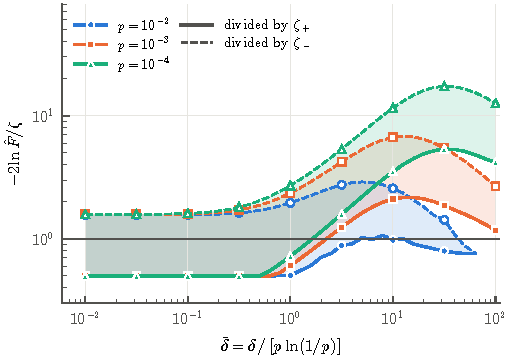
\includegraphics[width=0.6\linewidth]{figS2_fidelity_ratio}
\caption{The same bracket as Fig.~\ref{gate:fig:crossover}(a) for $-2\ln\Fg$, which is a Chernoff-type quantity and not itself a Stein converse. Solid lines divide by $\zeta_+$, dashed lines by $\zeta_-$.}
\label{gate:fig:Sfid}
\end{figure}

The remaining factor of at most $4.1$ between $\zeta_-$ and $\zeta_+$ is not attributed to either side: a strategy optimized for finite $\delta$ could raise $\zeta_-$, and more copies in the Fawzi--Fawzi hierarchy could lower $\zeta_+$. A search over Schmidt inputs $\sqrt q|00\rangle+\sqrt{1-q}|11\rangle$ found the maximally entangled input optimal at three test points.

\section{Biased Pauli noise and correlated miscalibrations}\label{gate:sec:biased}

This section applies Theorem~\ref{gate:thm:B} beyond uniform depolarizing noise. We treat (i) a single qubit with dephasing-dominated (biased) Pauli noise, as in bias-preserving architectures~\cite{Tuckett2018,Puri2020}, for $Z$ and $X$ miscalibrations; (ii) the asymptotic adaptive Fisher information $\Iinf$ for every Pauli channel and every Pauli-string miscalibration, in closed form; and (iii) the resulting local Stein bracket, including two qubits with a $ZZ$ miscalibration.

\emph{Setting.} A qubit Pauli channel has rates $q_\Id$, $p_x$, $p_y$, $p_z$ with $q_\Id=1-p_x-p_y-p_z$. Its bias ratio is $b=p_z/(p_x+p_y)$, so that depolarizing noise has $b=\frac12$. In the examples $p_x=p_y=p_\perp=p_z/(2b)$. The gate is $\cN_\delta=\mathcal P_q\circ\mathrm{Ad}_{R_P(\delta)}\circ\mathrm{Ad}_U$ as in Eq.~\eqref{gate:eq:Sgate}. In the notation of Theorem~\ref{gate:thm:B}, label the pairs $\{Q,QP\}$ by $k$, with rates $(q_k,q_k')$, and put
\begin{equation}\label{gate:eq:Bpair}
T_k=q_k+q_k',\qquad \Gamma_k=\frac{4q_kq_k'}{q_k+q_k'},\qquad \Gamma=\sum_k\Gamma_k ,
\end{equation}
so that $\sum_kT_k=1$, $0\le\Gamma_k\le T_k$ and $(q_k-q_k')^2=T_k(T_k-\Gamma_k)$. Pairs with $T_k=0$ are omitted. The pair containing the identity is $k=1$, $\{\Id,P\}$, with rates $(q_\Id,q_P)$; we call $q_P$ the \emph{coupled rate} of the miscalibration. For a qubit the second pair consists of the two Paulis other than $\Id$ and $P$. For $P=Z$ the pairs are $\{\Id,Z\}$ and $\{X,Y\}$; for $P=X$ they are $\{\Id,X\}$ and $\{Y,Z\}$.

\subsection*{Closed forms and the window}

\begin{proposition}[Biased qubit]\label{gate:prop:Bqubit}
Let $s=\sin(\delta/2)$, $q_\Id=1-p_z-2p_\perp$, and let $x_k=(q_k-q_k')^2s^2/(4q_kq_k')$ as in Eq.~\eqref{gate:eq:Sx}.
\begin{enumerate}
\item[(a)] For a $Z$ miscalibration the pair $\{X,Y\}$ has $x=0$, and for all $\delta$
\begin{gather}
\Fg=(1-2p_\perp)(1+x_1)^{-1/2}+2p_\perp,\qquad \DBS=2(1-2p_\perp)\varphi(x_1),\notag\\
x_1=\frac{(q_\Id-p_z)^2s^2}{4q_\Id p_z},\\
D=s^2(q_\Id-p_z)\ln\frac{q_\Id}{p_z},\qquad F=2p_\perp+\sqrt{(1-2p_\perp)^2-(q_\Id-p_z)^2s^2}.
\end{gather}
\item[(b)] For an $X$ miscalibration both pairs contribute:
\begin{gather}
\Fg=\frac{q_\Id+p_\perp}{\sqrt{1+x_1}}+\frac{p_z+p_\perp}{\sqrt{1+x_2}},\notag\\
x_1=\frac{(q_\Id-p_\perp)^2s^2}{4q_\Id p_\perp},\quad x_2=\frac{(p_z-p_\perp)^2s^2}{4p_zp_\perp},\\
\DBS=2(q_\Id+p_\perp)\varphi(x_1)+2(p_z+p_\perp)\varphi(x_2),\notag\\
D=s^2\Big[(q_\Id-p_\perp)\ln\frac{q_\Id}{p_\perp}+(p_z-p_\perp)\ln\frac{p_z}{p_\perp}\Big],\\
F=\sqrt{(q_\Id+p_\perp)^2-(q_\Id-p_\perp)^2s^2}+\sqrt{(p_z+p_\perp)^2-(p_z-p_\perp)^2s^2}.
\end{gather}
\item[(c)] In both cases, with the per-use Fisher informations
\begin{equation}\label{gate:eq:Bfisher}
\begin{gathered}
\IR=\sum_k\frac{T_k(T_k-\Gamma_k)}{\Gamma_k},\qquad \IB=\frac12\sum_k(q_k-q_k')\ln\frac{q_k}{q_k'},\\
\IS=\sum_k(T_k-\Gamma_k)=1-\Gamma ,
\end{gathered}
\end{equation}
one has, as $\delta\to0$,
\begin{gather}
-2\ln\Fg=\tfrac{\delta^2}{4}\IR+O(\delta^4/p_\perp^2),\qquad \DBS=\tfrac{\delta^2}{2}\IR+O(\delta^4/p_\perp^2),\\
D=\tfrac{\delta^2}{2}\IB+O(\delta^4\ln\tfrac1{p_\perp}),\qquad 1-F=\tfrac{\delta^2}{8}\IS+O(\delta^4).
\end{gather}
For a $Z$ miscalibration $\IR=(1-2p_\perp)(q_\Id-p_z)^2/(4q_\Id p_z)=\frac1{4p_z}[1+O(p_z)]$ and $\IB=\frac12(q_\Id-p_z)\ln(q_\Id/p_z)$. For an $X$ miscalibration $\IR=\frac{(q_\Id+p_\perp)(q_\Id-p_\perp)^2}{4q_\Id p_\perp}+\frac{(p_z+p_\perp)(p_z-p_\perp)^2}{4p_zp_\perp}=\frac{1}{4p_\perp}[1+O(p_z)]$ and $\IB=\frac12[\ln\frac1{p_\perp}+p_z\ln(2b)][1+O(p_z)]$.
\end{enumerate}
\end{proposition}

\begin{proof}
(a) and (b) are Theorem~\ref{gate:thm:B} with the pairs listed above; the maximally entangled input is optimal for $D$ and $F$. (c) follows from $g(x)=\frac x2+O(x^2)$, $\varphi(x)=x+O(x^2)$, $s^2=\frac{\delta^2}{4}+O(\delta^4)$ and $\sum_kT_kx_k=\frac{s^2}{4}\sum_kT_k(q_k-q_k')^2/(q_kq_k')$, together with $(q-q')^2=T(T-\Gamma)$ and $4qq'=\Gamma T$. Every $x_k$ is at most $s^2/(4\min_Qq_Q)$, which gives the remainders. The coefficients agree with Proposition~\ref{gate:prop:H}(v).
\end{proof}

\begin{proposition}[Window for any Pauli noise]\label{gate:prop:Bwindow}
Let $\cN_\delta$ be as in Eq.~\eqref{gate:eq:Sgate} on $n$ qubits with $q_\Id>q_P>0$, let $T_1=q_\Id+q_P$, and let $\delta_\eta=\inf\{\delta:1-\Fg(\cN_\delta,\cN_0)\ge\eta\}$.
\begin{enumerate}
\item[(a)] $T_1\,g(x_1)\le1-\Fg\le T_1\,g(x_1)+(1-T_1)$, with equality on the left when every pair other than $\{\Id,P\}$ has $q_k=q_k'$.
\item[(b)] Put $\delta(y)=2\arcsin\big(2\sqrt{q_\Id q_Py}/(q_\Id-q_P)\big)$ and $x_\eta=(1-\eta)^{-2}-1$. Then $\delta_\eta\le\delta\big(g^{-1}(\eta/T_1)\big)$, and, if $\eta>1-T_1$, $\delta_\eta\ge\delta\big(g^{-1}((\eta-1+T_1)/T_1)\big)$. In particular
\begin{equation}\label{gate:eq:Bwindow}
\delta_\eta=4\sqrt{x_\eta\,q_P/q_\Id}\,\big[1+O(1-T_1)+O(q_P)\big].
\end{equation}
\end{enumerate}
The window is therefore set by the coupled rate $q_P$. For local depolarizing noise $q_P/q_\Id=[p/(4-3p)]^w$, which recovers Theorem~\ref{gate:thm:W}(c). For $\DBS$, the inequality $\DBS\ge2T_1\varphi(x_1)$ gives the analogous upper bound on its window, and at fixed ratios of the rates the other pairs change the $\DBS$ window only by a relative $O(1-T_1)$.
\end{proposition}

\begin{proof}
By Theorem~\ref{gate:thm:B}, $1-\Fg=\sum_kT_kg(x_k)$ with $0\le g<1$; keep the first term, or bound the others by $\sum_{k\ge2}T_k=1-T_1$. Since $x_1$ is increasing in $\delta\in[0,\pi]$, inverting $g$ and solving $x_1=y$ for $\delta$ gives (b). As $1-T_1\to0$, both arguments of $g^{-1}$ tend to $\eta$, and $2\sqrt{q_\Id q_P}/(q_\Id-q_P)=2\sqrt{q_P/q_\Id}\,[1+O(q_P)]$.
\end{proof}

\begin{remark}[Floor and window are set by different rates]\label{gate:rem:Bfloor}
For $Z$-biased noise with $p_\perp<p_z$, the Choi floor is $\ltil=p_\perp$ whatever the miscalibration, so the worst-case modulus (Theorem~\ref{gate:thm:floor}) is $d/(4\lambda)=1/(4\ltil)=1/(4p_\perp)$. The window of a specific miscalibration is instead set by its coupled rate. A $Z$ miscalibration couples to $p_z$, the largest rate: $\delta_{0.1}=1.937\sqrt{p_z}$, independent of the bias. An $X$ miscalibration couples to $p_x=p_\perp$: $\delta_{0.1}=1.937\sqrt{p_z/(2b)}$, which narrows as $b^{-1/2}$. At $p_z=10^{-3}$ and $b=100$ the two windows are $6.14\times10^{-2}$ and $4.34\times10^{-3}$ rad for $\Fg$, and $2.88\times10^{-2}$ and $2.04\times10^{-3}$ rad for $\DBS$ (Fig.~\ref{gate:fig:biased}(a)). Pairs that do not contain the identity carry total weight $1-T_1\le p_x+p_y+p_z$ and only shift the window at that order. If such a pair has exactly one vanishing rate, the two Choi matrices have different supports, and $\DBS=D=\zeta=\infty$ for every $\delta\ne0$. If the coupled rate itself vanishes ($q_P=0$), the window closes; for example, an $X$ miscalibration under pure dephasing has $\Fg(\cN_\delta,\cN_0)=0$ for every $\delta\ne0$.
\end{remark}

\subsection*{Asymptotic adaptive Fisher information for Pauli channels}

\begin{theorem}[Adaptive QFI of a Pauli-string rotation under Pauli noise]\label{gate:thm:Bzj}
Let $\cN_\theta=\mathcal P_q\circ\mathrm{Ad}_{R_P(\theta)}\circ\mathrm{Ad}_U$ on $n$ qubits, with $\Gamma$ as in Eq.~\eqref{gate:eq:Bpair}.
\begin{enumerate}
\item[(a)] If $\Gamma=0$, the Hamiltonian-not-in-Kraus-span condition holds and the optimal $N$-use Fisher information grows as $N^2$. If $\Gamma>0$ it fails, and
\begin{equation}\label{gate:eq:Bzj}
\Iinf=\frac{1-\Gamma}{\Gamma},\qquad F_1=1-\Gamma=\IS ,
\end{equation}
where $F_1$ is the single-use entanglement-assisted Fisher information.
\item[(b)] If all $q_Q>0$, then $\IR=\sum_kT_k^2/\Gamma_k-1$ and
\begin{equation}\label{gate:eq:Bratio}
\frac{\IR}{\Iinf}=\frac{\Gamma}{1-\Gamma}\Big(\sum_k\frac{T_k^2}{\Gamma_k}-1\Big)\ \ge\ 1,
\end{equation}
with equality if and only if $\Gamma_k/T_k$ is the same for all pairs.
\end{enumerate}
For a qubit with $P=Z$, Eq.~\eqref{gate:eq:Bzj} is Eq.~(50) of Ref.~\cite{ZhouJiang2021}, which reads $\Gamma=4[p_xp_y/(p_x+p_y)+q_\Id p_z/(q_\Id+p_z)]$.
\end{theorem}

\begin{proof}
Since $\Iinf$ and $F_1$ do not depend on the Kraus representation, take $K_Q=\sqrt{q_Q}\,Q\,U$ for each Pauli string $Q$ with $q_Q>0$, and $K_{QP}=\sqrt{q_{QP}}\,QPU$ for its partner, using the operator $QP$ itself including its phase. Then $\dot K_Q=-\frac i2\sqrt{q_Q}\,QPU$, and $U$ drops out of every quantity below. The generator is $H=i\sum_QK_Q^\dagger\dot K_Q=P/2$.

(a, scaling) $K_Q^\dagger K_{Q'}$ is proportional to the Pauli string $QQ'$, which is proportional to $P$ only if $Q'\propto QP$. So $P/2$ lies in the Hermitian span of $\{K_Q^\dagger K_{Q'}\}$ if and only if some pair has both rates positive, that is, iff $\Gamma>0$. The scaling statement is Thm.~1 of Ref.~\cite{ZhouJiang2021}.

(a, value) By Thm.~2 of Ref.~\cite{ZhouJiang2021}, $\Iinf=4\min_{h:\beta(h)=0}\|\alpha(h)\|_\infty$ with $\alpha=\sum_QA_Q^\dagger A_Q$, $A_Q=\dot K_Q-i\sum_{Q'}h_{QQ'}K_{Q'}$ and $\beta=i\sum_QK_Q^\dagger A_Q$.

\emph{Lower bound.} Since $\|\alpha\|_\infty\ge\Tr\alpha/d$, and the Pauli strings are orthogonal in the Hilbert--Schmidt product, $\Tr\alpha/d$ is a sum of nonnegative terms. An entry $h_{QQ'}$ with $Q'\notin\{Q,QP\}$ enters $\Tr\alpha/d$ only through the term $q_{Q'}|h_{QQ'}|^2$, and enters $\beta$ only along Pauli strings other than $\Id$ and $P$. The constant part $i\sum K^\dagger\dot K=P/2$ has no such component. Setting these entries to zero therefore keeps $\beta=0$ feasible and does not increase the objective, so it suffices to minimize over $h$ supported on the pairs. Write the entries of pair $k$ as $h_{QQ}=u$, $h_{QP,QP}=v$ and $h_{Q,QP}=(y+ie)/(2\sqrt{q_kq_k'})$. A direct computation gives that the pair contributes
\begin{equation}
a_k\Id+a'_kP\ \text{to}\ \alpha,\qquad a_k=\frac{T_k}{4}+y+\frac{y^2+e^2}{\Gamma_k}+q_ku^2+q_k'v^2,
\end{equation}
and $(q_ku+q_k'v)\Id+(\frac{T_k}{2}+y)P$ to $\beta$, with $a'_k=0$ when $u=v=0$. For a pair with exactly one vanishing rate, $y$ is absent and $a_k\ge T_k/4$. Hence
\begin{equation}
\min_{\beta=0}\frac{\Tr\alpha}{d}=\min\Big\{\sum_k\Big(\frac{T_k}4+y_k+\frac{y_k^2}{\Gamma_k}\Big):\ \sum_ky_k=-\frac12\Big\}=\frac14-\frac12+\frac1{4\Gamma}=\frac{1-\Gamma}{4\Gamma},
\end{equation}
attained at $y_k=-\Gamma_k/(2\Gamma)$ and $u=v=e=0$.

\emph{Upper bound.} At this minimizer every $a'_k=0$, so $\alpha=\frac{1-\Gamma}{4\Gamma}\Id$ and $\|\alpha\|_\infty=\Tr\alpha/d$. This gives $\Iinf=(1-\Gamma)/\Gamma$.

Dropping the constraint $\sum_ky_k=-\frac12$ gives $y_k=-\Gamma_k/2$, $\alpha=\frac{1-\Gamma}4\Id$ and $F_1=4\min_h\|\alpha\|_\infty=1-\Gamma$. This coincides with $\IS$ at the maximally entangled input, by Theorem~\ref{gate:thm:B} and Eq.~\eqref{gate:eq:Bfisher}.

(b) The formula for $\IR$ is Eq.~\eqref{gate:eq:Bfisher} with $\sum_kT_k=1$. The inequality is Cauchy--Schwarz, $\sum_kT_k^2/\Gamma_k\ge(\sum_kT_k)^2/\sum_k\Gamma_k=1/\Gamma$, with equality iff $T_k/\Gamma_k$ is constant.
\end{proof}

Physically, $\IR$ sees mainly the coupled rate, $\IR\simeq1/\Gamma_1\simeq1/(4q_P)$, whereas $\Iinf\simeq1/\Gamma$ is limited by every pair whose two Pauli errors both occur. As the total error $1-q_\Id\to0$ at fixed ratios of the rates,
\begin{equation}\label{gate:eq:Bratio0}
\frac{\IR}{\Iinf}=1+\sum_{k\ge2}\frac{\Gamma_k}{\Gamma_1}+O(1-q_\Id).
\end{equation}
For a qubit this is $1+\frac{q_aq_b}{(q_a+q_b)q_P}$, where $q_a,q_b$ are the two spectator rates. The ratio is not bounded over Pauli channels: for an $X$ miscalibration with $p_x\ll p_y=p_z$ it is $1+p_y/(2p_x)$.

\subsection*{Local Stein bracket}

\begin{corollary}[Local Stein bracket for Pauli noise]\label{gate:cor:Bstein}
In the setting of Theorem~\ref{gate:thm:Bzj} with all $q_Q>0$,
\begin{equation}\label{gate:eq:Bbracket}
\liminf_{\delta\to0}\frac{\zeta(\cN_\delta\|\cN_0)}{\delta^2}\ge\frac{\Iinf}2=\frac{1-\Gamma}{2\Gamma},\qquad 1\le\limsup_{\delta\to0}\frac{\DBS(\cN_\delta\|\cN_0)}{\zeta(\cN_\delta\|\cN_0)}\le\frac{\IR}{\Iinf}.
\end{equation}
\end{corollary}

\begin{proof}
This is the argument of Proposition~\ref{gate:prop:local}. The constant-support hypothesis holds because, for all~$\delta$, $J(\cN_\delta)$ is unitarily equivalent to $J(\cN_0)$, whose smallest eigenvalue is $2^n\min_Qq_Q>0$. For every $N$-use strategy with outputs $\rho_N^\delta$, one has $\zeta\ge D(\rho_N^\delta\|\rho_N^0)/N$~\cite{WangWilde2019,FFRS2020}, and Proposition~\ref{gate:prop:H}(ii) gives $D=\frac{\delta^2}{2}F^{\rm BKM}+O(\delta^3)\ge\frac{\delta^2}{2}F^{\rm SLD}+O(\delta^3)$. Taking $N\to\infty$ over optimal strategies gives $\Iinf$ (Theorem~\ref{gate:thm:Bzj}). The upper side is $\zeta\le\DBS=\frac{\delta^2}2\IR+O(\delta^3)$ (Proposition~\ref{gate:prop:H}(v)).
\end{proof}

\emph{Biased qubit.} For a $Z$ miscalibration with $p_x=p_y=p_\perp$, Eq.~\eqref{gate:eq:Bratio} simplifies exactly to
\begin{equation}\label{gate:eq:BRZ}
\frac{\IR}{\Iinf}=T_1+\frac{p_\perp T_1^2}{2q_\Id p_z},\qquad T_1=1-2p_\perp,
\end{equation}
which equals $(2-p)(3-2p)/(4-3p)$ (Proposition~\ref{gate:prop:local}) at $p_\perp=p_z=p/4$. It satisfies $\IR/\Iinf<\frac32$ whenever $p_\perp\le p_z$ (i.e., $b\ge\frac12$) and $q_\Id>p_z$. To see this, set $t=p_\perp/p_z\in(0,1]$ and $\sigma=2(p_z+p_\perp)\in(0,1)$. Then $\frac32-\IR/\Iinf$ has the sign of $-[2t(t+1)\sigma^2-(4t^2+2t-1)\sigma+2t^2-2]$, which is convex in $\sigma$ and negative at $\sigma=0$ (for $t<1$) and at $\sigma=1$; at $t=1$ the bracket equals $\sigma(4\sigma-5)<0$. As $p_z\to0$ at fixed bias, $\IR/\Iinf=1+\frac1{4b}+O(p_z)$. Bias toward the rotation axis thus closes the bracket.

For pure dephasing ($p_\perp=0$) the range of $J(\cN_\delta)$, $\mathrm{span}\{\vect\Id,\vect Z\}$, does not depend on $\delta$. The argument of Corollary~\ref{gate:cor:Bstein} applies on this support, and $\DBS=2\varphi(x_1)$ exactly, so
\begin{equation}\label{gate:eq:Bdeph}
\lim_{\delta\to0}\frac{\zeta(\cN_\delta\|\cN_0)}{\delta^2}=\frac{\Iinf}2=\frac{\IR}2=\frac{(1-2p_z)^2}{8p_z(1-p_z)}.
\end{equation}
Here the local Stein coefficient is known exactly, and it coincides with the curvature of $\DBS$.

For an $X$ miscalibration under the same noise the spectator pair $\{Y,Z\}$ has $\Gamma_2\simeq4p_\perp$, comparable to $\Gamma_1\simeq4p_\perp$. Equation~\eqref{gate:eq:Bratio0} then gives $\IR/\Iinf\to(1+4b)/(1+2b)\in[\frac32,2)$, so the ratio $3/2$ is exceeded for every $b>\frac12$. The exact ratio stays below $2$ on a 30-digit grid of $22\,952$ points covering $p_\perp/p_z\in[10^{-6},1]$ and $2(p_z+p_\perp)\in[10^{-7},0.9999]$, with maximum $1.9999988$; we have no proof of this bound. In this case $\zeta/\delta^2\ge\Iinf/2\simeq1/(16p_\perp)$ for $b\gg1$, so the narrow window of Remark~\ref{gate:rem:Bfloor} also reflects a genuine sensitivity of $\zeta$, with $\DBS$ larger by at most a factor $2$. Table~\ref{gate:tab:Sbiased} lists values.

\begin{table}[!tbp]
\centering
\caption{Biased qubit noise with $p_z=10^{-3}$ and $p_x=p_y=p_z/(2b)$. The first two columns after $b$ give the windows of $\Fg$ ($1-\Fg=0.1$) and of $\DBS$ ($\DBS=0.1$). The local coefficients are $\DBS/\delta^2\to\IR/2$ and $\zeta/\delta^2\ge\Iinf/2$. All entries are exact evaluations of closed forms.}
\label{gate:tab:Sbiased}
\small
\begin{tabular}{llcccccc}
\toprule
$b$ & rotation & $\delta_{0.1}(\Fg)$ & $\delta_{0.1}(\DBS)$ & $\IR/2$ & $\Iinf/2$ & $\IR/\Iinf$ & $\IB$\\
\midrule
$\frac12$ & $Z$ or $X$ & $6.15\times10^{-2}$ & $2.89\times10^{-2}$ & 124.1 & 82.89 & 1.4975 & 3.44\\
$10$ & $Z$ & $6.14\times10^{-2}$ & $2.88\times10^{-2}$ & 124.6 & 121.6 & 1.0249 & 3.45\\
$10$ & $X$ & $1.37\times10^{-2}$ & $6.44\times10^{-3}$ & 2494 & 1280 & 1.9487 & 4.95\\
$100$ & $Z$ & $6.14\times10^{-2}$ & $2.88\times10^{-2}$ & 124.6 & 124.3 & 1.0025 & 3.45\\
$100$ & $X$ & $4.34\times10^{-3}$ & $2.04\times10^{-3}$ & $2.495\times10^{4}$ & $1.253\times10^{4}$ & 1.9911 & 6.10\\
$1000$ & $Z$ & $6.14\times10^{-2}$ & $2.88\times10^{-2}$ & 124.6 & 124.6 & 1.0002 & 3.45\\
$1000$ & $X$ & $1.37\times10^{-3}$ & $6.44\times10^{-4}$ & $2.495\times10^{5}$ & $1.250\times10^{5}$ & 1.9955 & 7.25\\
\bottomrule
\end{tabular}
\end{table}

\emph{Correlated miscalibrations.} For local depolarizing noise and $P$ of weight $w$, the quantities of Theorem~\ref{gate:thm:Bzj} depend on $w$ but not on $n$. The reason is that qubits outside the support of $P$ multiply both rates of a pair by the same factor. As $p\to0$,
\begin{equation}\label{gate:eq:Bweight}
\IR=\tfrac14(4/p)^w[1+O(p)],\qquad \Iinf=\Theta\big(p^{-\lceil w/2\rceil}\big),\qquad \IR/\Iinf=\Theta\big(p^{-\lfloor w/2\rfloor}\big).
\end{equation}
The leading term of $\Gamma$ comes from the pairs $\{Q,QP\}$ in which $Q$ and $QP$ each have weight about $w/2$ on the support of $P$. For example, for $P=Z\otimes Z$ the weight-one errors $Z\otimes\Id$ and $\Id\otimes Z$ form a pair with $\Gamma_k\simeq p/2$, whereas the coupled pair $\{\Id,ZZ\}$ has $\Gamma_1\simeq p^2/4$. For two qubits this gives
\begin{equation}\label{gate:eq:BZZ}
\Iinf=\frac2p[1+O(p)],\qquad \IR=\frac4{p^2}[1+O(p)],\qquad \frac{\IR}{\Iinf}=\frac2p[1+O(p)],
\end{equation}
so Corollary~\ref{gate:cor:Bstein} pins $\zeta/\delta^2$ only to $[1/p,\,2/p^2]$ to leading order. Table~\ref{gate:tab:Sweight} gives the limits for $w\le4$. Under $Z$-biased local noise ($p_z=10^{-3}$, $b=100$) a $ZZ$ miscalibration gives $\Iinf=498.5$ and $\IR/\Iinf=499.5\simeq1/(2p_z)$. This is controlled by the weight-one $Z$ errors and is no better than in the depolarizing case.

\begin{table}[!tbp]
\centering
\caption{Leading coefficients of $\Iinf$, $\IR$ and their ratio for local depolarizing noise and a miscalibration $Z^{\otimes w}$ (any $n\ge w$). Values are exact closed forms at $p=10^{-5}$, scaled as indicated; the limits are $2/3,1,3/2$ ($w=1$), $2,4,2$ ($w=2$), $2/3,16,24$ ($w=3$) and $8/3,64,24$ ($w=4$).}
\label{gate:tab:Sweight}
\begin{tabular}{lccc}
\toprule
$w$ & $p^{\lceil w/2\rceil}\Iinf$ & $p^w\IR$ & $p^{\lfloor w/2\rfloor}\IR/\Iinf$\\
\midrule
1 & 0.666658 & 0.999983 & 1.499994\\
2 & 1.999945 & 3.999880 & 1.999995\\
3 & 0.666667 & 15.99928 & 23.99892\\
4 & 2.666529 & 63.99616 & 23.99980\\
\bottomrule
\end{tabular}
\end{table}

Whether the true local coefficient of $\zeta$ for a weight-two error follows $\Iinf/2\sim1/p$ or $\IR/2\sim2/p^2$ is open. Explicit sequential strategies give $\Theta(1/p)$, but their relative-entropy rate is not known to be optimal. Until this is settled, the $p^{w/2}$ window of $\DBS$ for $w\ge2$ (Theorem~\ref{gate:thm:W}) is not known to be a property of $\zeta$.

\emph{Numerical verification.}
\begin{itemize}
\item The closed forms of Proposition~\ref{gate:prop:Bqubit} agree with direct 40-digit evaluations from $4\times4$ Choi matrices to within $1.2\times10^{-33}$ relative. The checks covered 24 points with $Z$ and $X$ miscalibrations, symmetric and asymmetric transverse rates, and Choi floors down to $4\times10^{-8}$. Maximally entangled inputs beat 40 random inputs for $D$ and $F$.
\item All $60$ exact windows (40-digit bisection) lie within the bounds of Proposition~\ref{gate:prop:Bwindow}, and their ratio to Eq.~\eqref{gate:eq:Bwindow} lies in $[1.006,1.024]$, $[1.0006,1.0024]$ and $[1.00006,1.00024]$ at $p_z=10^{-2}$, $10^{-3}$ and $10^{-4}$.
\item For the qubit we certified $\Iinf$ at $29$ biased points, including asymmetric $p_x\ne p_y$ and pure dephasing, with the method of Proposition~\ref{gate:prop:local}: a 50-digit minimax lower bound over the full $h$, and $\|\alpha\|_\infty$ at the minimizer. The two agree with each other and with Eq.~\eqref{gate:eq:Bzj} to within $10^{-46}$ relative, and the double-precision interior-point solution agrees to within $2\times10^{-7}$.
\item For two qubits ($16$ Kraus operators, input dimension $4$) we used double-precision interior-point solutions; the within-pair minimizer evaluated in 40 digits, for which $\beta=0$ to $10^{-36}$ and $\alpha\propto\Id$; and a double-precision lower bound over the full $16\times16$ matrix $h$. These agree with Eq.~\eqref{gate:eq:Bzj} to within $5\times10^{-6}$, $4\times10^{-36}$ and $2\times10^{-12}$ relative, respectively, for $ZZ$ at $p=10^{-1},\dots,10^{-4}$, for $Z\otimes\Id$, and for $ZZ$ and $XX$ under biased noise.
\item In every case $\IR$ computed as $\lmax\Tr_{\mathcal Y}[\dot JJ^{-1}\dot J]$ agrees with Eq.~\eqref{gate:eq:Bfisher} to within $10^{-33}$, and $\Tr_{\mathcal Y}[\cdot]$ is proportional to $\Id$.
\end{itemize}

\section{Certification}\label{gate:sec:cert-proofs}

\begin{proof}[Proof of Theorem~\ref{gate:thm:cert}]
The estimates are assumed to be channels, so $\Phi-\hat\Phi$ and $\Psi-\hat\Psi$ are trace annihilating and the constant $d_X/2$ of Lemma~\ref{gate:lem:J} applies. On the success event, Lemma~\ref{gate:lem:J} gives $\|J(\Phi)-J(\hat\Phi)\|_\infty\le r\hat\lambda$, so Weyl's inequality gives $\lambda(\Phi)\ge(1-r)\hat\lambda$, and $J(\hat\Phi)\ge\hat\lambda\Id$ gives $(1-r)J(\hat\Phi)\le J(\Phi)\le(1+r)J(\hat\Phi)$; likewise for $\Psi$. Joint monotonicity and degree-one homogeneity of $(A,B)\mapsto A\#_sB$ give $J(\Psi)\#_sJ(\Phi)\ge(1-r)\,J(\hat\Psi)\#_sJ(\hat\Phi)$ for every $s$, hence $\hat Q_s(\Phi\|\Psi)\ge(1-r)\hat Q_s(\hat\Phi\|\hat\Psi)$, and the minimum over $s$ gives Eq.~\eqref{gate:eq:cert}. The inequality $\xi\le\hat C$ is Theorem~\ref{chn:thm:main} in Chapter~\ref{chn:chapter}, and Corollary~\ref{gate:smp:cor:finite} gives the finite-$n$ bound with $\Lambda\le d_T(\hat\Phi,\hat\Psi)+2\ln\frac1{1-r}$.
\end{proof}

\emph{Stein version.} On the same event, Eq.~\eqref{gate:eq:Sstein} at the base pair $(\hat\Phi,\hat\Psi)$ with $\epsilon'\le\epsilon/2$, together with $\zeta(\hat\Phi\|\hat\Psi)\le\DBS(\hat\Phi\|\hat\Psi)$, gives
\begin{equation}
\zeta(\Phi\|\Psi)\le\DBS(\hat\Phi\|\hat\Psi)+\ln\frac1{1-r}+\epsilon\ln d_Y+\Big(1+\frac\epsilon2\Big)h\Big(\frac{\epsilon}{2+\epsilon}\Big)+\frac\epsilon2\ln\kappa(\hat\Psi),
\end{equation}
in which every term is computable from the estimates.

\emph{Sharpness of the radius.} By Eq.~\eqref{gate:eq:sharp}, there are model pairs and members of the diamond ball of radius $\epsilon$ whose values of $-\ln\Fg$ differ by $\frac{d_X\epsilon}{4\lambda}(1-o(1))$. A diamond-ball certificate with additive accuracy $\eta$ therefore needs $\epsilon\le4\eta\ltil(1+o(1))$.

\begin{proposition}[Cost through a diamond ball]\label{gate:prop:N12}
(a) With a known lower bound $\ltil_0\le\ltil$ and diamond-norm tomography~\cite{MeleBittel2025} at $\epsilon=\eta\ltil_0$, Theorem~\ref{gate:thm:cert} certifies $\hat C$ and $-\ln\Fg$ to additive accuracy $\eta\le1$ with $N=O\big((d_Xd_Yk+d_X\ln(1/\alpha))/(\eta\ltil_0)^2\big)$ uses per channel, where $1-\alpha$ is the confidence level. This learner processes the channel outputs coherently. (b) Consider learners that prepare a fresh input (with ancilla) for each use and measure the output, possibly choosing later inputs from earlier outcomes. Any such learner that outputs $\hat\Lambda$ with $\dn{\hat\Lambda-\cN_{p,\theta}}\le\epsilon$ with probability at least $2/3$ for all $\theta$ needs $N\ge0.0589\,(1-p)^2\epsilon^{-2}(1-o(1))$ uses.
\end{proposition}

\begin{proof}[Proof of (b)]
Two hypotheses $\theta,\theta'$ with $\dn{\cN_{p,\theta}-\cN_{p,\theta'}}=2(1-p)\sin\frac{|\theta-\theta'|}{2}=2\epsilon(1+o(1))$ must be distinguished with errors at most $1/3$. For classically adaptive kernels, the Bhattacharyya coefficient of the outcome records is at least the product of the per-round minima, each of which is at least the channel root fidelity, equal to its Choi value by Theorem~\ref{gate:thm:B}, i.e., at least $1-\sin^2\frac{\theta-\theta'}{2}$. Errors at most $1/3$ require a coefficient at most $\sqrt{8/9}$, which gives the bound with $0.0589=\frac12\ln\frac98$.
\end{proof}

\begin{remark}[Learner classes]\label{gate:rem:coherent}
Part (a) is achieved by a coherent learner and part (b) bounds incoherent learners, so Proposition~\ref{gate:prop:N12} does not establish a cost of order $1/(\eta\ltil)^2$ within a single learner class. For coherent learners the two-point argument on the family $\cN_{p,\theta}$ gives much less: with error-corrected probing the Fisher information per use for $\theta$ is at most $\Iinf=2(1-p)^2/[p(3-2p)]\approx2/(3p)$ (Sec.~\ref{gate:sec:local}), so distinguishing $\theta,\theta'$ with $|\theta-\theta'|\approx\epsilon/(1-p)$ requires only $N\gtrsim1/(\Iinf\epsilon^2)\approx3p/(2\epsilon^2)$, which at $\epsilon=4\eta\ltil=\eta p$ is of order $1/(\eta^2p)$, the order of the intrinsic cost of Proposition~\ref{gate:prop:N34}. Whether diamond-ball certification costs order $1/(\eta\ltil)^2$ uses for coherent learners is open.
\end{remark}

\begin{proposition}[Intrinsic cost]\label{gate:prop:N34}
(a) Let $\Psi_0=\Dp^{\otimes n}\circ\mathrm{Ad}_U$, and let $\Psi_1$ be the Pauli channel obtained by multiplying $q_P$ ($\mathrm{wt}P=n$, so $q_P=\ltil$) by $[(1+\eta)/(1-\eta)]^2$ and decreasing $q_\Id$ accordingly. Any $N$-use strategy, adaptive or coherent and with arbitrary quantum memory, that estimates $\Fg(\mathrm{Ad}_{PU},\Psi)$ to relative accuracy better than $\eta$ (i.e., with $|\hat f-\Fg|<\eta\Fg$ for its estimate $\hat f$) with probability at least $2/3$ under both hypotheses needs $N\ge c_0/(\eta^2\ltil)$, with $c_0=0.0246$ for $\eta\le0.1$, $p\le0.04$. (b) Preparing Bell pairs, applying the channel, undoing the known $U$ and measuring in the Bell basis, $N=\lceil3\ln(2/\alpha)/(\eta^2\ltil)\rceil$ uses estimate $q_P$, hence $\Fg(\mathrm{Ad}_{PU},\Psi)=\sqrt{q_P}$, to relative accuracy $(1\pm\eta)$ with probability at least $1-\alpha$.
\end{proposition}

\begin{proof}
(a) A Pauli channel is a mixture of unitaries, so the final state of any strategy is $\Lambda(q^{\otimes N})$ for a channel $\Lambda$ independent of $q$. Under the two hypotheses $\Fg=\sqrt{q_P}$ and $\Fg=\sqrt{q_P}\,(1+\eta)/(1-\eta)$, so the two open acceptance intervals $\{|\hat f-\Fg|<\eta\Fg\}$ are disjoint, and a successful estimator yields a test with both errors at most $1/3$, and data processing gives $N\,\mathrm{KL}(q^{(0)}\|q^{(1)})\ge\frac{\ln2}{3}$. The minimum of $N\eta^2\ltil$ over $\eta\in[0.005,0.1]$ and $p\in[10^{-6},0.04]$ is $0.02465$; analytically $\mathrm{KL}\le\chi^2\le16\eta^2\ltil(1+O(\eta+\ltil))$. The rank-one formula of Sec.~\ref{gate:sec:floor} gives $\Fg(\mathrm{Ad}_{PU},\Psi_j)=\sqrt{q_P^{(j)}}$. (b) Multiplicative Chernoff bound for a binomial with mean $Nq_P$.
\end{proof}

The perturbation in (a) changes the Pauli rates in the low-probability sector, where the information per use is $(\Delta q)^2/q\approx\eta^2\ltil$, not $\eta^2\ltil^2$. A two-point lower bound of order $1/(\eta\ltil)^2$ for the certification task itself is therefore false at this instance; the quadratic cost belongs to certification through a diamond ball. Hypothesis-testing quantities are different: the hockey-stick channel divergence satisfies $|E^\diamond_\gamma(\Phi'\|\Psi')-E^\diamond_\gamma(\Phi\|\Psi)|\le\frac12\dn{\Phi-\Phi'}+\frac\gamma2\dn{\Psi-\Psi'}$, so additive accuracy $\eta$ needs only $\epsilon\le2\eta/(1+\gamma)$, independently of $\lambda$.

\begin{conjecture}\label{gate:conj:cert}
For every channel pair with floor $\ltil$, the optimal number of uses for certifying $\hat C$ or $\Fg$ to relative accuracy $\eta$ is $\tilde\Theta(\mathrm{poly}(d)/(\eta^2\ltil))$.
\end{conjecture}

\emph{Simulations.} We simulated standard single-qubit Pauli process tomography (six input states, three measurement bases, 18 binary settings, exact binomial sampling) for the pair $\cN_{p,\delta}$, $\cN_{p,0}$ with $U=H$ and $\delta=2\sqrt p$, where $\Fg\approx0.71$. All confidence regions hold simultaneously with probability at least $0.95$ (Hoeffding or Clopper--Pearson bounds with a union bound).

\emph{Converse side.} A converse is certified by a lower confidence bound on $\Fg$ (an upper bound on $\hat C=-\ln\Fg$ for this pair) and an upper confidence bound on $\DBS$. We compared two procedures. (a) Linear inversion, which is exactly trace preserving, with the Hoeffding trace-norm ball $\|J_i-J_{\mathrm{LI},i}\|_1\le\epsilon_{\rm tr}$; Theorem~\ref{gate:thm:cert} then gives $\Fg\ge(1-r)\Fg(J_{\mathrm{LI},1},J_{\mathrm{LI},0})$ with $r=\epsilon_{\rm tr}/(2\hat\lambda)$, and the bound is vacuous if $r\ge1$. (b) Direct estimation of the Pauli error rates in the known frame (three settings per channel: prepare $U^\dagger|P_+\rangle$ and measure $P$), with Clopper--Pearson intervals defining a polytope of Pauli channels. Because $\Fg$ is jointly concave and $\DBS$ jointly convex while the Choi pair is affine in the rates, the minimum of $\Fg$ and the maximum of $\DBS$ over the product polytope are attained at pairs of vertices and were computed exactly by vertex enumeration. Procedure (b) assumes that the noise is a Pauli channel in the known frame. The accuracy target was $\ln(\Fg_{\rm true}/\Fg_{\rm LCB})\le\eta$ in the median run, on a grid of $1/8$ decade with 100 runs (a) or 50 runs (b) per point.

\begin{table}[!tbp]
\centering
\caption{Converse side: total channel uses per channel for a certified lower bound on $\Fg$ (and, for (b), an upper bound on $\DBS$) at accuracy $\eta=0.05$, median run, with fitted exponents $a$ in $N\propto p^{-a}$ and bootstrap 95\% intervals. The last row is the reference scale $c_0/(\eta^2\ltil)$ of Proposition~\ref{gate:prop:N34}(a), which is proved for the estimand $\Fg(\mathrm{Ad}_{PU},\Psi)$ at success probability $2/3$, not for the simulated pair with the median-run criterion.}
\label{gate:tab:Scert}
\footnotesize
\setlength{\tabcolsep}{3pt}
\begin{tabular}{lcccccc}
\toprule
procedure & $p=10^{-2}$ & $3\times10^{-3}$ & $10^{-3}$ & $3\times10^{-4}$ & $10^{-4}$ & $a$\\
\midrule
(a) diamond ball, Thm.~\ref{gate:thm:cert}, $\Fg$ & $3.6\times10^{11}$ & $4.0\times10^{12}$ & $3.6\times10^{13}$ & $4.0\times10^{14}$ & $3.6\times10^{15}$ & $2.000$\\
(b) Pauli rates, $\Fg$ & $1.2\times10^{6}$ & $4.3\times10^{6}$ & $1.2\times10^{7}$ & $3.9\times10^{7}$ & $1.2\times10^{8}$ & $1.00\,[0.99,1.03]$\\
(b) Pauli rates, $\DBS$ & $1.0\times10^{7}$ & $3.5\times10^{7}$ & $1.0\times10^{8}$ & $3.5\times10^{8}$ & $1.0\times10^{9}$ & $1.00\,[0.97,1.03]$\\
reference $c_0/(\eta^2\ltil)$ & $3.9\times10^{3}$ & $1.3\times10^{4}$ & $3.9\times10^{4}$ & $1.3\times10^{5}$ & $3.9\times10^{5}$ & $1$\\
\bottomrule
\end{tabular}
\end{table}

The ratio of (a) to (b) is about $750/\ltil$ at every $p$. The $p^{-2}$ of (a) holds by construction: the requirement $r=\epsilon_{\rm tr}/(2\lmin)\le\eta$ with $\lmin=p/2$, $\epsilon_{\rm tr}=36t$ and the Hoeffding width $t=[\ln(1440)/(2N_{\rm set})]^{1/2}$ alone gives $N=18\cdot36^2\ln(1440)/(2\eta^2p^2)\approx3.4\times10^7/p^2$ uses per channel, against $3.6\times10^7/p^2$ observed. The fitted exponents in $N\propto\eta^{-b}$ over $\eta\in\{0.1,0.05,0.025\}$ are $b=1.94$ for (a) and $1.65$--$1.76$ for (b), below the asymptotic value $2$ because these widths are pre-asymptotic. Procedure (a) lies a constant factor of about $1.5\times10^6$ above the incoherent-learner bound of Proposition~\ref{gate:prop:N12}(b) at the sharp radius $\epsilon=4\eta\ltil$, which reflects the constants of a non-optimal learner, not a different scaling. Procedure (b) assumes that both channels are Pauli channels in the known frame. On the converse side, the exact lower confidence bound over the model-free Clopper--Pearson box (a$''$) below is a concave minimization that we did not attempt, so whether model-free tomography attains the $1/\ltil$ law for certifying the converse is open. Procedure (b) lies a $p$-independent factor of about $300$ above the reference scale $c_0/(\eta^2\ltil)$; since that scale is proved for a different estimand and success criterion, this factor is not a gap to a lower bound for the simulated pair. Coverage, measured in 1000 runs per $p$ at the budget of each procedure, was $1.000$ (Clopper--Pearson interval $[0.996,1]$) for every certified bound; the median certified $\Fg$ was $0.67$--$0.68$ against a true value of $0.71$. At $\delta=1$, where $E_1\approx0.48$ and $F\approx0.88$, the hockey-stick divergence (upper bound $\frac12\dn{\hat\Phi-\hat\Psi}+\epsilon_{\rm tr}$) and the Uhlmann fidelity (lower bound through the purified distance) were certified through the same ball with $3.4\times10^{7}$ and $5.9\times10^{10}$ uses, independently of $p$ (fitted slopes $0.000$ and $-0.008$).

\emph{Opposite side.} Upper bounds on $\Fg$ and lower bounds on $\DBS$, which limit distinguishability from below, are convex programs over the confidence region; we solved them with a safety margin of $10^{-5}$ above the solver tolerance, using the geometric R\'enyi divergence of order $7/8$ (monotone in the order) for $\DBS$. We used four regions: (a) the trace-norm ball, (a$'$) a Hoeffding box on the 18 setting probabilities, (a$''$) a Clopper--Pearson box, i.e., exact binomial intervals per setting with no model assumption, and (b) the known-frame Pauli polytope. With the criterion that the certified divergence lies within a factor two of the truth (median of 10 runs), the total uses per channel at $p=10^{-3}$ were $4.3\times10^{10}$, $1.3\times10^{9}$, $9.4\times10^{6}$ and $2.4\times10^{5}$, with fitted exponents $1.98$, $1.93$, $0.96$ and $0.99$ over $p\in[10^{-4},10^{-2}]$, the same range as Table~\ref{gate:tab:Scert}. A variance-adaptive region thus removes the extra factor $1/\ltil$ without any model assumption, while the variance-blind regions (a) and (a$'$) do not. For the box and ball regions, 1000 repetitions at $(p,N)=(10^{-2},10^6)$, $(10^{-3},10^8)$ and $(10^{-4},10^{10})$ shots per setting gave coverage $1.000$ against a nominal $0.95$. At the same sample sizes, and at $(p,N)=(10^{-3},10^{10})$, the plug-in $\Fg$ from linear inversion exceeded the truth, which makes the converse claim a stronger limit than is true, in $21.8\%$, $8.2\%$, $0.6\%$ and $31.9\%$ of runs. A hedged maximum-likelihood estimate~\cite{BlumeKohout2010} with $\beta=1/2$ did so in up to $96\%$ of runs at $10^2$--$10^3$ shots per setting ($p\le10^{-3}$). A route that uses only the different-sums continuity bound of Theorem~\ref{cont:thm:four maps} in Chapter~\ref{cont:chapter} with a Weyl-certified floor did not become non-vacuous below $10^{12}$ shots per setting.

\emph{Two qubits.} For a CNOT gate with a $Z\otimes Z$ miscalibration under local noise, plug-in estimation of $\Fg$ to $10\%$ accuracy in $90\%$ of runs (product Pauli tomography, linear inversion with projection onto channels) needed $10^6$, $10^8$ and $10^{10}$ shots per setting at $p=0.1$, $0.03$ and $0.01$, i.e., $N\approx p^{-4}$ on a one-decade grid with three points, consistent with $1/\lambda^2$ and $\lambda=p^2/4$. These are plug-in estimates, not certified bounds.

\section{Numerical methods}\label{gate:sec:methods}

Geometric means were computed through the Arveson--Radon--Nikodym factorization of the pair, which is stable when both Choi matrices are invertible, and cross-checked against semidefinite programs. Closed forms were verified against direct matrix computations in 40--60-digit arithmetic (\texttt{mpmath}); semidefinite programs used \texttt{cvxpy} with Clarabel, with SCS as a cross-check. Diamond norms used the Watrous semidefinite program~\cite{watrous2018theory}. Whenever a Choi eigenvalue fell below $10^{-8}$, finite differences were evaluated in multiple-precision arithmetic, because square roots of round-off-level eigenvalues corrupt double-precision derivatives. The code, random seeds and raw data are in the \texttt{code/} directory of the repository that accompanies this book, \url{https://github.com/mjones1298/Continuity-of-divergences-python-}; its \texttt{README.md} lists the script and output file behind each number of this chapter and of Chapter~\ref{gate:chapter}.

\section{\texorpdfstring{Refinements of results from Chapters~\ref{cont:chapter}, \ref{shA:chapter} and~\ref{chn:chapter}}{Refinements of results from other chapters}}\label{gate:smp:sec}

The continuity of the geometric quantities, the Thompson-metric and first-argument continuity of the adaptive Stein exponent, the geometric Chernoff converse and the program-simulation converse, which Sections~\ref{gate:sec:regimes}--\ref{gate:sec:cert} of Chapter~\ref{gate:chapter} and Sections~\ref{gate:sec:floor}, \ref{gate:sec:ad} and~\ref{gate:sec:cert-proofs} of this chapter use, are proved in Chapters~\ref{cont:chapter}, \ref{shA:chapter} and~\ref{chn:chapter}. This section points to them and proves, for finite-dimensional channels, the refinements that are needed here and are not proved there. Maps act from $\mathrm L(\mathcal X)$ to $\mathrm L(\mathcal Y)$ and are completely positive (CP), and channels when stated. We use $\Tr_{\mathcal Y}J(\Lambda)=\Lambda^*(\Id)^T$, so that $\Tr_{\mathcal Y}J(\Phi)=\Id$ for a channel, and $\Tr_{\mathcal Y}|\vect A\rangle\langle\vect B|=(B^\dagger A)^T$.

\emph{Kubo--Ando facts.} For $s\in(0,1)$ and positive semidefinite (PSD) $A,B$ we use only the following properties of $\#_s$~\cite{KuboAndo1980}. (K1) $\#_s$ is monotone in each argument. (K2) $(aA)\#_s(bB)=a^{1-s}b^s\,A\#_sB$ for $a,b>0$. (K3) $X(A\#_sB)X^\dagger=(XAX^\dagger)\#_s(XBX^\dagger)$ for invertible $X$, and $A\#_sB=A^{1-s}B^s$ for commuting $A,B>0$. (K4) $\#_s$ is continuous on pairs of positive definite operators, and $A_n\#_sB_n\to A\#_sB$ whenever $A_n\downarrow A$ and $B_n\downarrow B$. (K5) $A\#_sB\le(1-s)A+sB$ and $A\#_sA=A$. By the defining formula and (K4), the mean of two block-diagonal pairs is block diagonal. With the convention of Sec.~\ref{gate:sec:notation}, $\hat Q_0=\hat Q_1=1$, and $\hat Q_s\le1$ for channels (proof of Theorem~\ref{chn:thm:semicont}(b)), so $e^{-\hat C}=\inf_{0<s<1}\hat Q_s$; we use this form throughout.

\emph{Derivatives and levels.}
Let $\Phi,\Psi$ be CP maps and fix an injective $W$ with $WW^\dagger=J(\Phi+\Psi)$, whose columns are linearly independent Kraus operators of $\Phi+\Psi$. The derivative $T$ of $\Phi$ with respect to $\Phi+\Psi$ (Section~\ref{cont:sec:prelim}) satisfies $0\le T\le\Id$, $J(\Phi)=WTW^\dagger$ and $J(\Psi)=W(\Id-T)W^\dagger$. With $b_s(t)=t^s(1-t)^{1-s}$ and $b_s(0)=b_s(1)=0$ for $0<s<1$, Theorem~\ref{cont:fundamental principle} gives $J(\Psi)\#_sJ(\Phi)=W\,b_s(T)\,W^\dagger$, and Theorem~\ref{cont:range theorem} gives $\mathrm{ran}(A\#_sB)=\mathrm{ran}A\cap\mathrm{ran}B$ for PSD $A,B$. The levels $\tau_\ell$ of a pair of channels, the operators $S_\ell$ and $B_s$, the constant $\Lambda\le d_T(\Phi,\Psi)$ and the identity $\hat Q_s(\Phi\|\Psi)=\lmin(B_s)$ for $0<s<1$ are those of Section~\ref{chn:sec:levels} (Lemma~\ref{chn:lem:levels} and Remark~\ref{chn:rem:geom}, where $b_s$ is written $g_s$).

\subsection*{Continuity of the geometric quantities and the scope of the dichotomy}
$\hat Q_s$ and $\Fg$ are upper semicontinuous on pairs of CP maps (Lemma~\ref{cont:lem:envelope}(c)), and hence so is $e^{-\hat C}=\inf_{0<s<1}\hat Q_s$; in particular $\Fg$ and $\hat Q_s$ are continuous at every pair at which they vanish. As functions on pairs of CP maps, $\Fg$ and $\hat Q_s$ are continuous at $(\Phi,\Psi)$ if and only if $J(\Phi+\Psi)$ is invertible or $\Fg(\Phi,\Psi)=0$ (Theorem~\ref{cont:thm:dichotomy}(a) and (d)(ii)). Restricted to pairs of channels, $\Fg$ is continuous at $(\Phi,\Phi)$ if and only if $J(\Phi)$ is invertible, and if $J(\Phi)$ is singular the output rotations $\Phi_t=\mathrm{Ad}_{e^{-itH}}\circ\Phi$ witness the discontinuity for suitable Hermitian $H$ (Corollary~\ref{cont:cor:diagonal channels} and Theorem~\ref{cont:thm:channel orbit}(b)); whether the `only if' direction holds at off-diagonal channel pairs with $J(\Phi+\Psi)$ singular and $\Fg(\Phi,\Psi)>0$ is open (Section~\ref{cont:sec:conclusion}). For unitaries, $\Fg(\mathrm{Ad}_U,\mathrm{Ad}_{U'})=0$ whenever $U'\notin\mathbb CU$, while $\Fg(\mathrm{Ad}_U,\mathrm{Ad}_U)=1$ (Corollary~\ref{cont:cor:channels dichotomy}). For amplitude damping, $\mathrm{ran}J(\cA_\gamma)\cap\mathrm{ran}J(\cA_{\gamma'})\subseteq\mathrm{span}\{\vect|0\rangle\langle1|\}$ and $\Fg(\cA_\gamma,\cA_{\gamma'})=0$ for $\gamma\ne\gamma'$ in $[0,1]$ (Example~\ref{cont:ex:amplitude damping}), and $\hat C=-2\ln\Fg=C_{\rm bar}=+\infty$ for $0<\gamma,\gamma'\le1$ (Proposition~\ref{chn:prop:adlevels}). For pairs of channels, $\hat C$ is lower semicontinuous everywhere and continuous wherever $J(\Phi+\Psi)$ is invertible (Theorem~\ref{chn:thm:semicont}(a,c)). The following proposition extends the last statement to completely positive maps.

\begin{proposition}\label{gate:smp:prop:cont}
Let $\Phi,\Psi$ be CP maps and $0<s<1$. If $J(\Phi+\Psi)$ is invertible, then $\hat Q_s$, $\Fg$ and $\hat C$ are continuous at $(\Phi,\Psi)$.
\end{proposition}

\begin{proof}
Near $(\Phi,\Psi)$, $S'=J(\Phi'+\Psi')$ is invertible, and Theorem~\ref{cont:fundamental principle} with $W=S'^{1/2}$ gives $T'=S'^{-1/2}J(\Phi')S'^{-1/2}$, which is continuous in the pair, and $\hat Q_s(\Phi'\|\Psi')=\lmin\Tr_{\mathcal Y}(S'^{1/2}b_s(T')S'^{1/2})$. This is continuous for fixed $s$. For $\hat C$, since $e^{-\hat C}$ is upper semicontinuous, it remains to show $\liminf e^{-\hat C(\Phi',\Psi')}\ge e^{-\hat C(\Phi,\Psi)}$. Choose $\eta\in(0,\frac14)$ such that $T$ has no eigenvalue in $(0,2\eta)\cup(1-2\eta,1)$, and let $k_s$ equal $b_s$ on $[2\eta,1-2\eta]$, vanish on $[0,\eta]\cup[1-\eta,1]$ and be affine in between. Since $b_s$ is concave and nonnegative, $0\le k_s\le b_s$, and $k_s(T)=b_s(T)$. The family $\{k_s\}_{0<s<1}$ is uniformly bounded and equicontinuous, because $(s,t)\mapsto b_s(t)$ is uniformly continuous on $[0,1]\times[\eta,1-\eta]$, so it is totally bounded in the supremum norm (Arzel\`a--Ascoli). Approximating by a finite net shows $\sup_s\|k_s(T')-k_s(T)\|_\infty\to0$ as $T'\to T$. Hence $\hat Q_s(\Phi'\|\Psi')\ge\lmin\Tr_{\mathcal Y}(S'^{1/2}k_s(T')S'^{1/2})\to\lmin\Tr_{\mathcal Y}(S^{1/2}b_s(T)S^{1/2})=\hat Q_s(\Phi\|\Psi)$ uniformly in $s$, and taking the infimum over $s$ gives the claim.
\end{proof}

\subsection*{The two-sided Choi-floor law with separate floors}

\begin{proposition}\label{gate:smp:prop:twosided}
Let $\Phi,\Phi',\Psi,\Psi'$ be CP maps. Put $r_\Phi=\|J(\Phi')-J(\Phi)\|_\infty/\lambda(\Phi)$ if $\lambda(\Phi)>0$ and $r_\Phi=0$ if $\Phi'=\Phi$, define $r_\Psi$ likewise, and assume $r_\Phi,r_\Psi<1$. Then for $0<s<1$
\begin{equation}\label{gate:smp:eq:twosided}
(1-r_\Psi)^{1-s}(1-r_\Phi)^s\,\hat Q_s(\Phi\|\Psi)\le\hat Q_s(\Phi'\|\Psi')\le(1+r_\Psi)^{1-s}(1+r_\Phi)^s\,\hat Q_s(\Phi\|\Psi).
\end{equation}
In particular
\begin{gather*}
\sqrt{(1-r_\Phi)(1-r_\Psi)}\le\frac{\Fg(\Phi',\Psi')}{\Fg(\Phi,\Psi)}\le\sqrt{(1+r_\Phi)(1+r_\Psi)},\\
|\hat C(\Phi',\Psi')-\hat C(\Phi,\Psi)|\le\ln\frac1{1-\max\{r_\Phi,r_\Psi\}}.
\end{gather*}
With $\lambda=\min\{\lambda(\Phi),\lambda(\Psi)\}$ and $\eta_J$ as in Sec.~\ref{gate:sec:floor}, the equal-floor bounds $1\pm\eta_J/\lambda$, for $\Fg$ and for every Kubo--Ando connection, are Theorem~\ref{cont:thm:choi floor}(a,b).
For channels, $\eta_J/\lambda\le r=d_X\epsilon/(2\lambda)$ with $\epsilon=\max\{\dn{\Phi'-\Phi},\dn{\Psi'-\Psi}\}$, by Lemma~\ref{gate:lem:J}.
\end{proposition}

\begin{proof}
$J(\Phi)\ge\lambda(\Phi)\Id$ gives $(1-r_\Phi)J(\Phi)\le J(\Phi)-r_\Phi\lambda(\Phi)\Id\le J(\Phi')\le J(\Phi)+r_\Phi\lambda(\Phi)\Id\le(1+r_\Phi)J(\Phi)$, and likewise for $\Psi$. Apply (K1) and (K2), and use that $Z\mapsto\lmin\Tr_{\mathcal Y}Z$ is monotone and positively homogeneous.
\end{proof}

For $\Phi'=\Phi$ this is Eq.~\eqref{gate:eq:floor}. Since $\Fg$ is symmetric, Eq.~\eqref{gate:eq:sharp} shows that each of the two terms is sharp separately, when the other channel is unitary and therefore has floor $0$. Whether the constant $d_X/(2\lambda)$ for $\ln\Fg$ is attained when both channels move and both floors are at least $\lambda$ is open.

\subsection*{The Thompson metric and the adaptive Stein exponent}

An $n$-use adaptive strategy consists of a state $\rho_1$ on $\mathcal X\otimes\mathcal R_1$, channels $\Gamma_k:\mathrm L(\mathcal Y\otimes\mathcal R_k)\to\mathrm L(\mathcal X\otimes\mathcal R_{k+1})$ for $k<n$, and a final measurement on $\mathcal Y\otimes\mathcal R_n$. Its final states are $\rho^\Phi_n=(\Phi\otimes\mathrm{id})\Gamma_{n-1}\cdots\Gamma_1(\Phi\otimes\mathrm{id})(\rho_1)$ and $\rho^\Psi_n$. We use $\zeta(\Phi\|\Psi)=D^{\rm reg}(\Phi\|\Psi)=\lim_n\frac1nD(\Phi^{\otimes n}\|\Psi^{\otimes n})=D^A(\Phi\|\Psi)$~\cite{WangWilde2019,FFRS2020}. Here $D$ of channels is the Umegaki channel divergence, and $D^A(\Phi\|\Psi)=\sup[D((\mathrm{id}\otimes\Phi)\rho\|(\mathrm{id}\otimes\Psi)\sigma)-D(\rho\|\sigma)]$ is the amortized divergence, with the supremum over finite-dimensional $\mathcal R$ and states $\rho,\sigma$ on $\mathcal R\otimes\mathcal X$ with $D(\rho\|\sigma)<\infty$. We write $\kappa(\Psi)=\lmax(J(\Psi))/\lmin(J(\Psi))$ and $h$ for the binary entropy.

The Choi sandwich $\lmin(J(\Psi))\,\sigma_{\mathcal R}\otimes\Id\le(\mathrm{id}\otimes\Psi)(\sigma)\le\lmax(J(\Psi))\,\sigma_{\mathcal R}\otimes\Id$ is Lemma~\ref{shA:lem:sandwichchoi}. If $J(\Psi)\le c\,J(\Psi')$, then $\rho^\Psi_n\le c^n\rho^{\Psi'}_n$ for every $n$-use adaptive strategy (Lemma~\ref{shA:lem:order}). Consequently, for every divergence that is antitone in its second argument and satisfies $\mathbb D(\rho\|c\sigma)=\mathbb D(\rho\|\sigma)-\ln c$, such as the Umegaki, Belavkin--Staszewski or max-relative entropy, the suprema over adaptive or parallel $n$-use strategies are $n\,d_T$-Lipschitz in $\Psi$, and $|\zeta(\Phi\|\Psi)-\zeta(\Phi\|\Psi')|\le d_T(\Psi,\Psi')$ (Theorem~\ref{shA:thm:thompson}). With Eq.~\eqref{gate:eq:Ssandwich}, $d_T(\Psi,\Psi')\le\ln\frac1{1-r}$ for $r=d_X\dn{\Psi-\Psi'}/(2\lambda(\Psi))<1$; the constant $d_X/2$ of Lemma~\ref{gate:lem:J} halves the radius used in Theorem~\ref{shA:thm:thompson}. The first-argument bound for $D$ and $D^A$, uniformly over references, is Theorem~\ref{shA:thm:firstarg}. Corollary~\ref{shA:cor:stein} gives the properties of $\zeta$ used here: $\zeta$ is lower semicontinuous on pairs of channels; if $J(\Psi)$ is invertible, then $\zeta(\Phi\|\Psi)\le\ln(d_X/\lambda(\Psi))$ and Eq.~\eqref{gate:eq:Sstein} holds; and $\zeta$ is continuous at $(\Phi,\Psi)$ if and only if $J(\Psi)$ is invertible or $\zeta(\Phi\|\Psi)=\infty$.

\begin{remark}\label{gate:smp:rem:zeta}%
If $J(\Phi+\Psi)$ is invertible, then either $J(\Psi)$ is invertible or $\mathrm{ran}J(\Phi)\not\subseteq\mathrm{ran}J(\Psi)$, in which case $\zeta(\Phi\|\Psi)\ge D(\Phi\|\Psi)=\infty$. So $\zeta$, too, is continuous at every pair with $J(\Phi+\Psi)$ invertible.
\end{remark}

\begin{remark}\label{gate:smp:rem:dbs}
$\DBS$ is continuous, with values in $(-\infty,+\infty]$, at every pair of CP maps with $J(\Phi+\Psi)$ invertible. Chapter~\ref{cont:chapter} does not state this as a single result; it follows from that chapter as follows, since $\DBS=\widehat D_f$ with $f(t)=t\ln t$, for which $f(0^+)=0$ and $f'(\infty)=+\infty$. Let $(\Phi',\Psi')\to(\Phi,\Psi)$. Their relative distance $\delta$ to $(\Phi,\Psi)$ tends to $0$ (Corollary~\ref{cont:cor:four maps cb}), and hence so do $\tau$ and $d_T$ (Lemma~\ref{cont:lem:one parameter}). If $J(\Psi)$ is invertible, then $J(\Psi')\ge\frac12\lmin(J(\Psi))\Id$ eventually, so $D_{\max}(\Phi'\|\Psi')$ is bounded uniformly, and Theorem~\ref{cont:thm:four maps}(e) gives $\DBS(\Phi'\|\Psi')\to\DBS(\Phi\|\Psi)$. If $J(\Psi)$ is singular, then $\mathrm{ran}J(\Phi)\not\subseteq\mathrm{ran}J(\Psi)$ and $\DBS(\Phi\|\Psi)=+\infty$ (Theorem~\ref{cont:thm:all f}(a)); a bound $J(\Phi')\le cJ(\Psi')$ along a subsequence with bounded $c$ would give $J(\Phi)\le cJ(\Psi)$ in the limit, so $D_{\max}(\Phi'\|\Psi')\to+\infty$, while $\nu(\Phi'+\Psi')$ stays bounded below by Lemma~\ref{cont:lem:nu}(2) and $\|(\Phi'+\Psi')^*(\Id)\|_\infty$ stays bounded, and Corollary~\ref{cont:cor:dmax growth} gives $\DBS(\Phi'\|\Psi')\to+\infty$. Theorem~\ref{cont:thm:extended continuity} is the corresponding statement for perturbations with a fixed sum $\Phi+\Psi$, along which it holds at every pair.
\end{remark}

\subsection*{The geometric Chernoff converse}

For an $n$-use adaptive strategy as above, the optimal error with equal priors is $P^{\rm err}_n=\frac12-\frac14\|\rho^\Phi_n-\rho^\Psi_n\|_1$, and $\xi(\Phi,\Psi)=\limsup_n-\frac1n\ln\inf P^{\rm err}_n$, the infimum running over strategies.

Every adaptive protocol is a controlled random walk on the levels of the pair (Proposition~\ref{chn:prop:walk}). For every pair of channels, every $n\ge1$ and every $n$-use adaptive strategy, $P^{\rm err}_n\ge\tfrac14\exp\big(-n\hat C(\Phi,\Psi)-\sqrt{2\ln4}\,\Lambda\sqrt n\big)$ with $\Lambda\le d_T(\Phi,\Psi)$, so that $\xi(\Phi,\Psi)\le\hat C(\Phi,\Psi)$ (Theorem~\ref{chn:thm:main}); moreover $-\ln\Fg(\Phi,\Psi)\le\hat C(\Phi,\Psi)\le-2\ln\Fg(\Phi,\Psi)$ (Corollary~\ref{chn:cor:compare}(a)).

\begin{corollary}[Finite-$n$ converse for an uncertain pair]\label{gate:smp:cor:finite}
On the success event of Theorem~\ref{gate:thm:cert}, every $n$-use adaptive strategy for the true pair has
\[
P^{\rm err}_n\ge\tfrac14\exp\Big(-n\Big[\hat C(\hat\Phi,\hat\Psi)+\ln\frac1{1-r}\Big]-\sqrt{2\ln4}\,\Big[d_T(\hat\Phi,\hat\Psi)+2\ln\frac1{1-r}\Big]\sqrt n\Big).
\]
\end{corollary}

\begin{proof}
The proof of Theorem~\ref{gate:thm:cert} (Sec.~\ref{gate:sec:cert-proofs}) gives $\hat C(\Phi,\Psi)\le\hat C(\hat\Phi,\hat\Psi)+\ln\frac1{1-r}$ and $(1-r)J(\hat\Phi)\le J(\Phi)\le(1+r)J(\hat\Phi)$, so $d_T(\Phi,\hat\Phi)\le\ln\frac1{1-r}$, and likewise for $\Psi$. The triangle inequality for $d_T$ and Theorem~\ref{chn:thm:main} with $\Lambda\le d_T(\Phi,\Psi)$ give the claim.
\end{proof}

\subsection*{Fragility of single-letter Chernoff converses}

Write $\xi_{\rm QC}(\phi,\psi)=-\ln\min_{0\le s\le1}\Tr\phi^s\psi^{1-s}$ for the quantum Chernoff exponent of two states~\cite{AudenaertChernoff2007,NussbaumSzkola2009}, and $\FU(\phi,\psi)=\|\sqrt\phi\sqrt\psi\|_1$ for their root fidelity.

Theorem~\ref{chn:thm:fragile} constructs replacement channels at distance $O(\sqrt t)$ from a given pair at which the three single-letter converses are infinite; the following version gives an explicit construction and distance.

\begin{theorem}[Replacement channels]\label{gate:smp:thm:fragile}
Let $\phi,\psi$ be states on $\mathbb C^{d'}$ with $\mathrm{rank}(\phi+\psi)\le d'/2$, and let $\Phi=\Tr(\cdot)\phi$, $\Psi=\Tr(\cdot)\psi$. There are states $\phi_t,\psi_t$ with $\|\phi_t-\phi\|_1,\|\psi_t-\psi\|_1\le2(\sqrt t+t)$ such that the replacement channels $\Phi_t=\Tr(\cdot)\phi_t$ and $\Psi_t=\Tr(\cdot)\psi_t$ satisfy, for every $t>0$,
\begin{gather*}
\hat C(\Phi_t,\Psi_t)=-2\ln\Fg(\Phi_t,\Psi_t)=C_{\rm bar}(\Phi_t,\Psi_t)=+\infty,\\
\xi(\Phi_t,\Psi_t)=\xi_{\rm QC}(\phi_t,\psi_t)\le-\ln\Tr\phi_t^{1/2}\psi_t^{1/2}\xrightarrow[t\to0]{}-\ln\Tr\phi^{1/2}\psi^{1/2}.
\end{gather*}
If $\phi=\psi$, then $\dn{\Phi_t-\Phi},\dn{\Psi_t-\Phi}\le2(\sqrt t+t)$ and $\xi(\Phi_t,\Psi_t)\to0$, while the three converses are infinite for every $t>0$.
\end{theorem}

\begin{proof}
Let $\mathcal K=\mathrm{supp}(\phi+\psi)$. Since $\dim\mathcal K\le d'/2$, there is a partial isometry $V$ with $V^\dagger V$ the projection onto $\mathcal K$ and $\mathrm{ran}V\subseteq\mathcal K^\perp$. Put $A_\pm=\Id\pm\sqrt tV$, $\phi_t=A_+\phi A_+^\dagger/(1+t)$ and $\psi_t=A_-\psi A_-^\dagger/(1+t)$. These are states, since $\Tr V\phi=0$ and $\Tr V\phi V^\dagger=1$. Also $\phi_t-\phi=[\sqrt t(V\phi+\phi V^\dagger)+t(V\phi V^\dagger-\phi)]/(1+t)$ has trace norm at most $2(\sqrt t+t)$, and likewise for $\psi_t$. If $A_+x=A_-y$ with $x,y\in\mathcal K$, the components in $\mathcal K$ and $\mathcal K^\perp$ give $x=y$ and $Vx=-Vy$, so $x=y=0$. Hence $\mathrm{ran}\phi_t\cap\mathrm{ran}\psi_t\subseteq A_+\mathcal K\cap A_-\mathcal K=\{0\}$, and so $\mathrm{ran}J(\Phi_t)\cap\mathrm{ran}J(\Psi_t)=(\mathrm{ran}\phi_t\cap\mathrm{ran}\psi_t)\otimes\mathcal X=\{0\}$, because $J(\Phi_t)=\phi_t\otimes\Id$. Theorem~\ref{cont:range theorem} gives $\hat Q_s(\Phi_t\|\Psi_t)=0$ for $0<s<1$, hence $\hat C=-2\ln\Fg=\infty$. For every channel $\mathcal T$, $J(\mathcal T)\ne0$ cannot have range in both $\mathrm{ran}J(\Phi_t)$ and $\mathrm{ran}J(\Psi_t)$, so, as in the proof of Theorem~\ref{chn:thm:semicont}(d), $C_{\rm bar}=\infty$. A replacement channel ignores its input, so the final states of every adaptive strategy are $\mathcal S(\phi_t^{\otimes n})$ and $\mathcal S(\psi_t^{\otimes n})$ for one channel $\mathcal S$. The strategy that measures the $n$ outputs is therefore optimal, and $\xi=\xi_{\rm QC}(\phi_t,\psi_t)$~\cite{AudenaertChernoff2007,NussbaumSzkola2009}. This is at most the value at $s=\frac12$, which is continuous in the states. Finally $\dn{\Tr(\cdot)(\phi_t-\phi)}=\|\phi_t-\phi\|_1$.
\end{proof}

\emph{The example of Fig.~\ref{gate:fig:regimes}(b).} For $\phi=\psi=\frac12(|1\rangle\langle1|+|2\rangle\langle2|)$ on $\mathbb C^4$ and $V=|3\rangle\langle1|+|4\rangle\langle2|$, the states $\phi_t=\frac12(v_+v_+^\dagger+w_+w_+^\dagger)$ and $\psi_t=\frac12(v_-v_-^\dagger+w_-w_-^\dagger)$, with $v_\pm=(|1\rangle\pm\sqrt t|3\rangle)/\sqrt{1+t}$ and $w_\pm=(|2\rangle\pm\sqrt t|4\rangle)/\sqrt{1+t}$, are block diagonal with pure blocks. For every $s\in[0,1]$, $\Tr\phi_t^s\psi_t^{1-s}=|\langle v_+,v_-\rangle|^2=(\frac{1-t}{1+t})^2$, so $\xi(\Phi_t,\Psi_t)=2\ln\frac{1+t}{1-t}$ exactly, and $\dn{\Phi_t-\Phi}=2\sqrt{t/(1+t)}$. The root fidelity is $\FU(\phi_t,\psi_t)=\frac{1-t}{1+t}$, so the program-simulation converse of Theorem~\ref{chn:thm:pureprog}, for which $\mu_*=\FU(\phi_t,\psi_t)$ at replacement channels (see the discussion after that theorem), is tight here: $-2\ln\mu_*(\Phi_t,\Psi_t)=\xi(\Phi_t,\Psi_t)$.

\subsection*{The program-simulation converse}
Parts (a)--(c) of the program-simulation converse quoted in Sec.~\ref{gate:sec:ad} are Theorem~\ref{chn:thm:pureprog}, whose fidelity is the square of the root fidelity $\FU$ used here. For replacement channels $\Phi=\Tr(\cdot)\phi$, $\Psi=\Tr(\cdot)\psi$ one has $\mu_*(\Phi,\Psi)=\FU(\phi,\psi)$, and $-2\ln\mu_*$ is finite along any approximating pairs of replacement channels and converges to its value at the limit pair, so $\min\{\hat C,C_{\rm bar},-2\ln\mu_*\}$ does not jump along the pairs of Theorem~\ref{gate:smp:thm:fragile} with $\phi=\psi$ (discussion after Theorem~\ref{chn:thm:pureprog}). For $0<\gamma,\gamma'\le1$, $\mu_*(\cA_\gamma,\cA_{\gamma'})=\sqrt{\gamma\gamma'}/(1-a)$ with $a=\sqrt{(1-\gamma)(1-\gamma')}$ (Corollary~\ref{chn:cor:adfragile}).


\endgroup
